% !TeX spellcheck = en-US
% !TeX encoding = utf8
% !TeX program = pdflatex
% !BIB program = biber
% -*- coding:utf-8 mod:LaTeX -*-
% !TEX root = ./main-english.tex

% vv  scroll down to line 200 for content  vv


\let\ifdeutsch\iffalse
\let\ifenglisch\iftrue
% EN: This file is loaded before the \documentclass command in the main document

% EN: The following package allows \\ at the title page
%     For more information see https://github.com/latextemplates/scientific-thesis-cover/issues/4
\RequirePackage{kvoptions-patch}

\ifenglisch
  \PassOptionsToClass{numbers=noenddot}{scrbook}
\else
  %()Aus scrguide.pdf - der Dokumentation von KOMA-Script)
  %Nach DUDEN steht in Gliederungen, in denen ausschließlich arabische Ziffern für die Nummerierung
  %verwendet werden, am Ende der Gliederungsnummern kein abschließender Punkt
  %(siehe [DUD96, R3]). Wird hingegen innerhalb der Gliederung auch mit römischen Zahlen
  %oder Groß- oder Kleinbuchstaben gearbeitet, so steht am Ende aller Gliederungsnummern ein
  %abschließender Punkt (siehe [DUD96, R4])
  \PassOptionsToClass{numbers=autoendperiod}{scrbook}
\fi

% Warns about outdated packages and missing caption declarations
% See https://www.ctan.org/pkg/nag
\RequirePackage[l2tabu, orthodox]{nag}

%DE: Neue deutsche Trennmuster
%    Siehe http://www.ctan.org/pkg/dehyph-exptl und http://projekte.dante.de/Trennmuster/WebHome
%    Nur für pdflatex, nicht für lualatex
\RequirePackage{ifluatex}
\ifluatex
  % do not load anything
\else
  \ifdeutsch
    \RequirePackage[ngerman=ngerman-x-latest]{hyphsubst}
  \fi
\fi

\documentclass[
  % fontsize=11pt is the standard
  a4paper,  % Standard format - only KOMAScript uses paper=a4 - https://tex.stackexchange.com/a/61044/9075
  twoside,  % we are optimizing for both screen and two-side printing. So the page numbers will jump, but the content is configured to stay in the middle (by using the geometry package)
  bibliography=totoc,
  %               idxtotoc,   %Index ins Inhaltsverzeichnis
  %               liststotoc, %List of X ins Inhaltsverzeichnis, mit liststotocnumbered werden die Abbildungsverzeichnisse nummeriert
  headsepline,
  cleardoublepage=empty,
  parskip=half,
  %               draft    % um zu sehen, wo noch nachgebessert werden muss - wichtig, da Bindungskorrektur mit drin
  draft=false
]{scrbook}
% !TeX encoding = utf8
% -*- coding:utf-8 mod:LaTeX -*-

% EN: This file includes basic packages and sets options. The order of package
%     loading is important

% DE: In dieser Datei werden zuerst die benoetigten Pakete eingebunden und
%     danach diverse Optionen gesetzt. Achtung Reihenfolge ist entscheidend!


% EN: Styleguide:
% - English comments are prefixed with "EN", German comments are prefixed with "DE"
% - Prefixed headings define the language for the subsequent paragraphs
% - It is tried to organize packages in blocks. Bocks are separated by two empty lines.

% DE: Styleguide:
%
% Ein sehr kleiner Styleguide. Packages werden in Blöcken organisiert.
% Zwischen zwei Blöcken sind 2 Leerzeilen!


% EN: Enable copy and paste of text from the PDF
%     Only required for pdflatex. It "just works" in the case of lualatex.
%     mmap enables mathematical symbols, but does not work with the newtx font set
%     See: https://tex.stackexchange.com/a/64457/9075
%     Other solutions outlined at http://goemonx.blogspot.de/2012/01/pdflatex-ligaturen-und-copynpaste.html and http://tex.stackexchange.com/questions/4397/make-ligatures-in-linux-libertine-copyable-and-searchable
%     Trouble shooting outlined at https://tex.stackexchange.com/a/100618/9075

\ifluatex
\else
  \usepackage{cmap}
\fi


% EN: File encoding
% DE: Codierung
%     Wir sind im 21 Jahrhundert, utf-8 löst so viele Probleme.
%
% Mit UTF-8 funktionieren folgende Pakete nicht mehr. Bitte beachten!
%   * fancyvrb mit §
%   * easylist -> http://www.ctan.org/tex-archive/macros/latex/contrib/easylist/
\ifluatex
  % EN: See https://tex.stackexchange.com/a/158517/9075
  %     Not required, because of usage of fontspec package
  %\usepackage[utf8]{luainputenc}
\else
  \usepackage[utf8]{inputenc}
\fi


% DE: Parallelbetrieb tex4ht und pdflatex

\makeatletter
\@ifpackageloaded{tex4ht}{
  \def\iftex4ht{\iftrue}
}{
  \def\iftex4ht{\iffalse}
}
\makeatother


% EN: Mathematics
% DE: Mathematik
%
% DE: Viele Mathematik-Sachen. Siehe https://texdoc.net/pkg/amsmath
%
% EN: Options must be passed this way, otherwise it does not work with glossaries
% DE: fleqn (=Gleichungen linksbündig platzieren) funktioniert nicht direkt. Es muss noch ein Patch gemacht werden:
\PassOptionsToPackage{fleqn,leqno}{amsmath}
%
% DE: amsmath Muss nicht mehr geladen werden, da es von newtxmath automatisch geladen wird
% \usepackage{amsmath}


%% EN: Fonts
%% DE: Schriften
%%
%% !!! If you change the font, be sure that words such as "workflow" can
%% !!! still be copied from the PDF. If this is not the case, you have
%% !!! to use glyphtounicode. See comment at cmap package


% EN: Times Roman for all text
\ifluatex
  \RequirePackage{amsmath}
  \RequirePackage{unicode-math}
  \setmainfont{TeX Gyre Termes}
  \setmathfont{texgyretermes-math.otf}
  \setsansfont[Scale=.9]{TeX Gyre Heros}
  \setmonofont[StylisticSet={1,3},Scale=.9]{inconsolata}
\else
  \RequirePackage{newtxtext}
  \RequirePackage{newtxmath}
  % EN: looks good with times, but no equivalent for lualatex found,
  %     therefore replaced with inconsolata
  %\RequirePackage[zerostyle=b,scaled=.9]{newtxtt}
  \RequirePackage[varl,scaled=.9]{inconsolata}

  % DE: Symbole
  % unicode-math scheint für die meisten schon etwas anzubieten
  %
  %\usepackage[geometry]{ifsym} % \BigSquare

  % EN: The euro sign
  % DE: Das Euro Zeichen
  %     Fuer Palatino (mathpazo.sty): richtiges Euro-Zeichen
  %     Alternative: \usepackage{eurosym}
  \newcommand{\EUR}{\ppleuro}
\fi


% DE: Noch mehr Symbole
%\usepackage{stmaryrd} %fuer \ovee, \owedge, \otimes
%\usepackage{marvosym} %fuer \Writinghand %patched to not redefine \Rightarrow
%\usepackage{mathrsfs} %mittels \mathscr{} schoenen geschwungenen Buchstaben erzeugen
%\usepackage{calrsfs} %\mathcal{} ein bisserl dickeren buchstaben erzeugen - sieht net so gut aus.

% EN: Fallback font - if the subsequent font packages do not define a font (e.g., monospaced)
%     This is the modern package for "Computer Modern".
%     In case this gets activated, one has to switch from cmap package to glyphtounicode (in the case of pdflatex)
% DE: Fallback-Schriftart
%\usepackage[%
%    rm={oldstyle=false,proportional=true},%
%    sf={oldstyle=false,proportional=true},%
%    tt={oldstyle=false,proportional=true,variable=true},%
%    qt=false%
%]{cfr-lm}

% EN: Headings are typset in Helvetica (which is similar to Arial)
% DE: Schriftart fuer die Ueberschriften - ueberschreibt lmodern
%\usepackage[scaled=.95]{helvet}

% DE: Für Schreibschrift würde tun, muss aber nicht
%\usepackage{mathrsfs} %  \mathscr{ABC}

% EN: Font for the main text
% DE: Schriftart fuer den Fliesstext - ueberschreibt lmodern
%     Linux Libertine, siehe http://www.linuxlibertine.org/
%     Packageparamter [osf] = Minuskel-Ziffern
%     rm = libertine im Brottext, Linux Biolinum NICHT als serifenlose Schrift, sondern helvet (von oben) beibehalten
%\usepackage[rm]{libertine}

% EN: Alternative Font: Palantino. It is recommeded by Prof. Ludewig for German texts
% DE: Alternative Schriftart: Palantino, Packageparamter [osf] = Minuskel-Ziffern
%     Bitte nur in deutschen Texten
%\usepackage{mathpazo} %ftp://ftp.dante.de/tex-archive/fonts/mathpazo/ - Tipp aus DE-TEX-FAQ 8.2.1

% DE: Schriftart fuer Programmcode - ueberschreibt lmodern
%     Falls auskommentiert, wird die Standardschriftart lmodern genommen
%     Fuer schreibmaschinenartige Schluesselwoerter in den Listings - geht bei alten Installationen nicht, da einige Fontshapes (<>=) fehlen
%\usepackage[scaled=.92]{luximono}
%\usepackage{courier}
% DE: BeraMono als Typewriter-Schrift, Tipp von http://tex.stackexchange.com/a/71346/9075
%\usepackage[scaled=0.83]{beramono}

% EN: backticks (`) are rendered as such in verbatim environments.
%     See following links for details:
%     - https://tex.stackexchange.com/a/341057/9075
%     - https://tex.stackexchange.com/a/47451/9075
%     - https://tex.stackexchange.com/a/166791/9075
\usepackage{upquote}

% EN: For \texttrademark{}
\usepackage{textcomp}

% EN: name-clashes von marvosym und mathabx vermeiden:
\def\delsym#1{%
  %  \expandafter\let\expandafter\origsym\expandafter=\csname#1\endcsname
  %  \expandafter\let\csname orig#1\endcsname=\origsym
  \expandafter\let\csname#1\endcsname=\relax
}

%\usepackage{pifont}
%\usepackage{bbding}
%\delsym{Asterisk}
%\delsym{Sun}\delsym{Mercury}\delsym{Venus}\delsym{Earth}\delsym{Mars}
%\delsym{Jupiter}\delsym{Saturn}\delsym{Uranus}\delsym{Neptune}
%\delsym{Pluto}\delsym{Aries}\delsym{Taurus}\delsym{Gemini}
%\delsym{Rightarrow}
%\usepackage{mathabx} - Ueberschreibt leider zu viel - und die \le-Zeichen usw. sehen nicht gut aus!


% EN: Modern font encoding
%     Has to be loaded AFTER any font packages. See https://tex.stackexchange.com/a/2869/9075.
\ifluatex
\else
  \usepackage[T1]{fontenc}
\fi
%


% EN: Character protrusion and font expansion. See http://www.ctan.org/tex-archive/macros/latex/contrib/microtype/
% DE: Optischer Randausgleich und Grauwertkorrektur

\usepackage[
  babel=true, % EN: Enable language-specific kerning. Take language-settings from the languge of the current document (see Section 6 of microtype.pdf)
  expansion=alltext,
  protrusion=alltext-nott, % EN: Ensure that at listings, there is no change at the margin of the listing
  final % EN: Always enable microtype, even if in draft mode. This helps finding bad boxes quickly.
        %     In the standard configuration, this template is always in the final mode, so this option only makes a difference if "pros" use the draft mode
]{microtype}


% EN: \texttt{test -- test} keeps the "--" as "--" (and does not convert it to an en dash)
\DisableLigatures{encoding = T1, family = tt* }

% DE: fuer microtype
% DE: tracking=true muss als Parameter des microtype-packages mitgegeben werden
% DE: Deaktiviert, da dies bei Algorithmen seltsam aussieht

%\DeclareMicrotypeSet*[tracking]{my}{ font = */*/*/sc/* }%
%\SetTracking{ encoding = *, shape = sc }{ 45 }
% DE: Hier wird festgelegt,
%     dass alle Passagen in Kapitälchen automatisch leicht
%     gesperrt werden.
%     Quelle: http://homepage.ruhr-uni-bochum.de/Georg.Verweyen/pakete.html
%    Deaktiviert, da sonst "BPEL", "BPMN" usw. wirklich komisch aussehen.
%     Macht wohl nur bei geisteswissenschaftlichen Arbeiten Sinn.


% EN: amsmath teaks


% EN: Fixes bugs in AMS math
%     Corrently conflicts with unicode-math
% \usepackage{mathtools}

%\numberwithin{equation}{section}
%\renewcommand{\theequation}{\thesection.\Roman{equation}}

% EN: work-around ams-math problem with align and 9 -> 10. Does not work with glossaries, No visual changes.
%\addtolength\mathindent{1em}


% EN: For theorems, replacement for amsthm
\usepackage[amsmath,hyperref]{ntheorem}
\theorempreskipamount 2ex plus1ex minus0.5ex
\theorempostskipamount 2ex plus1ex minus0.5ex
\theoremstyle{break}
\newtheorem{definition}{Definition}[section]


% CTAN: https://ctan.org/pkg/lccaps
% Doc: http://texdoc.net/pkg/lccaps
%
% Required for DE/EN \initialism
\usepackage{lccaps}


% EN: Defintion of colors. Argument "hyperref" is not used as we do not want to change border colors of links: Links are not colored anymore.
% DE: Farbdefinitionen
\usepackage[dvipsnames]{xcolor}


% EN: Required for custom acronyms/glossaries style.
%     Left aligned Columns in tables with fixed width.
%     See http://tex.stackexchange.com/questions/91566/syntax-similar-to-centering-for-right-and-left
\usepackage{ragged2e}


% DE: Wichtig, ansonsten erscheint "No room for a new \write"
\usepackage{scrwfile}


% EN: Support for language-specific hyphenation
% DE: Neue deutsche Rechtschreibung und Literatur statt "Literature"
%     Die folgende Einstellung ist der Nachfolger von ngerman.sty
\ifdeutsch
  % DE: letzte Sprache ist default, Einbindung von "american" ermöglicht \begin{otherlanguage}{amercian}...\end{otherlanguage} oder \foreignlanguage{american}{Text in American}
  %     Siehe auch http://tex.stackexchange.com/a/50638/9075
  \usepackage[american,main=ngerman]{babel}
  % Ein "abstract" ist eine "Kurzfassung", keine "Zusammenfassung"
  \addto\captionsngerman{%
    \renewcommand\abstractname{Kurzfassung}%
  }
  \ifluatex
    % EN: conditionally disable ligatures. See https://github.com/latextemplates/scientific-thesis-template/issues/54
    %     for a discussion
    \usepackage[ngerman]{selnolig}
  \fi
\else
  % EN: Set English as language and allow to write hyphenated"=words
  %     `american`, `english` and `USenglish` are synonyms for babel package (according to https://tex.stackexchange.com/questions/12775/babel-english-american-usenglish).
  %      "english" has to go last to set it as default language
  \usepackage[ngerman,main=english]{babel}
  % EN: Hint by http://tex.stackexchange.com/a/321066/9075 -> enable "= as dashes
  \addto\extrasenglish{\languageshorthands{ngerman}\useshorthands{"}}
  \ifluatex
    % EN: conditionally disable ligatures. See https://github.com/latextemplates/scientific-thesis-template/issues/54
    %     for a discussion
    \usepackage[english]{selnolig}
  \fi
\fi
%


% EN: For easy quotations: \enquote{text}
%     This package is very smart when nesting is applied, otherwise textcmds (see below) provides a shorter command
%     Note that this package results in a warning when it is loaded before minted (actually fvextra).
% DE: Anführungszeichen
%     Zitate in \enquote{...} setzen, dann werden automatisch die richtigen Anführungszeichen verwendet.
%     Dieses package erzeugt eine Warnung, wenn es vor minted (genauer fvextra) geladen wird.
\usepackage{csquotes}


% EN: For even easier quotations: \qq{text}.
%     Is not smart in the case of nesting, but good enough for the most cases
\usepackage{textcmds}
\ifdeutsch
  % EN: German quotes are different. So do not use the English quotes, but the ones provided by the csquotes package.
  \renewcommand{\qq}[1]{\enquote{#1}}
\fi


% EN: extended enumarations
% DE: erweitertes Enumerate
\usepackage{paralist}


% DE: Gestaltung der Kopf- und Fußteilen

\usepackage[automark]{scrlayer-scrpage}

\automark[section]{chapter}
\setkomafont{pageheadfoot}{\normalfont\sffamily}
\setkomafont{pagenumber}{\normalfont\sffamily}

% DE: funktioniert nicht: Alle Linien sind hier weg
%\setheadsepline[.4pt]{.4pt}


% DE: Intelligentes Leerzeichen um hinter Abkürzungen die richtigen Abstände zu erhalten, auch leere.
%     Siehe commands.tex \gq{}
\usepackage{xspace}
% DE: Macht \xspace und \enquote kompatibel
\makeatletter
\xspaceaddexceptions{\grqq \grq \csq@qclose@i \} }
\makeatother


\newcommand{\eg}{e.\,g.,\ }
\newcommand{\ie}{i.\,e.,\ }


% EN: introduce \powerset - hint by http://matheplanet.com/matheplanet/nuke/html/viewtopic.php?topic=136492&post_id=997377
\DeclareFontFamily{U}{MnSymbolC}{}
\DeclareSymbolFont{MnSyC}{U}{MnSymbolC}{m}{n}
\DeclareFontShape{U}{MnSymbolC}{m}{n}{
  <-6>    MnSymbolC5
  <6-7>   MnSymbolC6
  <7-8>   MnSymbolC7
  <8-9>   MnSymbolC8
  <9-10>  MnSymbolC9
  <10-12> MnSymbolC10
  <12->   MnSymbolC12%
}{}
\DeclareMathSymbol{\powerset}{\mathord}{MnSyC}{180}


% EN: Package for the appendix
% DE: Anhang
\usepackage{appendix}
%[toc,page,title,header]
%


% EN: Graphics
% DE: Grafikeinbindungen
%
% EN: The parameter "pdftex" is not required
\usepackage{graphicx}
\graphicspath{{\getgraphicspath}}
\newcommand{\getgraphicspath}{graphics/}


% EN: Enables inclusion of SVG graphics - 1:1 approach
%    This is NOT the approach of https://ctan.org/pkg/svg-inkscape,
%     which allows text in SVG to be typeset using LaTeX
%     We just include the SVG as is.
\usepackage{epstopdf}
\epstopdfDeclareGraphicsRule{.svg}{pdf}{.pdf}{%
  inkscape -z -D --file=#1 --export-pdf=\OutputFile
}


% EN: Enables inclusion of SVG graphics - text-rendered-with-LaTeX-approach
%     This is the approach of https://ctan.org/pkg/svg-inkscape,
\newcommand{\executeiffilenewer}[3]{%
  \IfFileExists{#2}
  {
    %\message{file #2 exists}
    \ifnum\pdfstrcmp{\pdffilemoddate{#1}}%
      {\pdffilemoddate{#2}}>0%
      {\immediate\write18{#3}}
    \else
      {%\message{file up to date #2}
      }
    \fi%
  }{
    %\message{file #2 doesn't exist}
    %\message{argument: #3}
    %\immediate\write18{echo "test" > xoutput.txt}
    \immediate\write18{#3}
  }
}
\newcommand{\includesvg}[1]{%
  \executeiffilenewer{#1.svg}{#1.pdf}%
  {
    inkscape -z -D --file=\getgraphicspath#1.svg %
    --export-pdf=\getgraphicspath#1.pdf --export-latex}%
  \input{\getgraphicspath#1.pdf_tex}%
}


% EN: Enable typesetting values with SI units.
\ifdeutsch
  \usepackage[mode=text,group-minimum-digits=4]{siunitx}
  \sisetup{locale=DE}
\else
  \usepackage[mode=text,group-minimum-digits=4,group-separator={,}]{siunitx}
  \sisetup{locale=US}
\fi


% EN: Extensions for tables
% DE: Tabellenerweiterungen
\usepackage{array} %increases tex's buffer size and enables ``>'' in tablespecs
\usepackage{longtable}
\usepackage{dcolumn} %Aligning numbers by decimal points in table columns
\ifdeutsch
  \newcolumntype{d}[1]{D{.}{,}{#1}}
\else
  \newcolumntype{d}[1]{D{.}{.}{#1}}
\fi
\setlength{\extrarowheight}{1pt}


% DE: Eine Zelle, die sich über mehrere Zeilen erstreckt.
%     Siehe Beispieltabelle in Kapitel 2
\usepackage{multirow}


% DE: Fuer Tabellen mit Variablen Spaltenbreiten
%\usepackage{tabularx}
%\usepackage{tabulary}


% EN: Links behave as they should. Enables "\url{...}" for URL typesettings.
%     Allow URL breaks also at a hyphen, even though it might be confusing: Is the "-" part of the address or just a hyphen?
%     See https://tex.stackexchange.com/a/3034/9075.
% DE: Links verhalten sich so, wie sie sollen
%     Zeilenumbrüche bei URLs auch bei Bindestrichen erlauben, auch wenn es verwirrend sein könnte: Gehört der Bindestrich zur URL oder ist es ein Trennstrich?
%     Siehe https://tex.stackexchange.com/a/3034/9075.
\usepackage[hyphens]{url}
%
%  EN: When activated, use text font as url font, not the monospaced one.
%      For all options see https://tex.stackexchange.com/a/261435/9075.
% \urlstyle{same}
%
% EN: Hint by http://tex.stackexchange.com/a/10419/9075.
\makeatletter
\g@addto@macro{\UrlBreaks}{\UrlOrds}
\makeatother


% DE: Index über Begriffe, Abkürzungen
%\usepackage{makeidx} makeidx ist out -> http://xindy.sf.net verwenden


% DE: lustiger Hack fuer das Abkuerzungsverzeichnis
%     nach latex durchlauf folgendes ausfuehren
%     makeindex ausarbeitung.nlo -s nomencl.ist -o ausarbeitung.nls
%     danach nochmal latex
%\usepackage{nomencl}
%    \let\abk\nomenclature %Deutsche Ueberschrift setzen
%          \renewcommand{\nomname}{List of Abbreviations}
%        %Punkte zw. Abkuerzung und Erklaerung
%          \setlength{\nomlabelwidth}{.2\hsize}
%          \renewcommand{\nomlabel}[1]{#1 \dotfill}
%        %Zeilenabstaende verkleinern
%          \setlength{\nomitemsep}{-\parsep}
%    \makenomenclature


% EN: Logic for TeX - enables if-then-else in commands
% DE: Logik für TeX
%     FÜr if-then-else @ commands.tex
\usepackage{ifthen}


% EN: Code Listings
% DE: Listings
\usepackage{listings}
\lstset{language=XML,
  showstringspaces=false,
  extendedchars=true,
  basicstyle=\footnotesize\ttfamily,
  commentstyle=\slshape,
  % DE: Original: \rmfamily, damit werden die Strings im Quellcode hervorgehoben. Zusaetzlich evtl.: \scshape oder \rmfamily durch \ttfamily ersetzen. Dann sieht's aus, wie bei fancyvrb
  stringstyle=\ttfamily,
  breaklines=true,
  breakatwhitespace=true,
  % EN: alternative: fixed
  columns=flexible,
  numbers=left,
  numberstyle=\tiny,
  basewidth=.5em,
  xleftmargin=.5cm,
  % aboveskip=0mm, %DE: deaktivieren, falls man lstlistings direkt als floating object benutzt (\begin{lstlisting}[float,...])
  % belowskip=0mm, %DE: deaktivieren, falls man lstlistings direkt als floating object benutzt (\begin{lstlisting}[float,...])
  captionpos=b
}

\ifluatex
\else
  % EN: Enable UTF-8 support - see https://tex.stackexchange.com/q/419327/9075
  \usepackage{listingsutf8}
  \lstset{inputencoding=utf8/latin1}
\fi

\ifdeutsch
  \renewcommand{\lstlistlistingname}{Verzeichnis der Listings}
\fi


% EN: Alternative to listings could be fancyvrb. Can be used together.
% DE: Alternative zu Listings ist fancyvrb. Kann auch beides gleichzeitig benutzt werden.
\usepackage{fancyvrb}
%
% EN: Font size for the normal text
% DE: Groesse fuer den Fliesstext. Falls deaktiviert: \normalsize
%\fvset{fontsize=\small}
%
% DE: Somit kann im Text ganz einfach §verbatim§ text gesetzt werden.
%     Disabled, because UTF-8 does not work any more and lualatex causes issues
%\DefineShortVerb{\§}
%
% EN: Shrink font size of listings
\RecustomVerbatimEnvironment{Verbatim}{Verbatim}{fontsize=\footnotesize}
\RecustomVerbatimCommand{\VerbatimInput}{VerbatimInput}{fontsize=\footnotesize}
%
% EN: Hack for fancyvrb based on http://newsgroups.derkeiler.com/Archive/Comp/comp.text.tex/2008-12/msg00075.html
%     Change of the solution: \Vref somehow collidated with cleveref/varioref as the output of \Vref{} was "Abschnitt 4.3 auf Seite 85"; therefore changed to \myVref -- so completely removed
%     See https://tex.stackexchange.com/q/132420/9075 for more information.
\newcommand{\Vlabel}[1]{\label[line]{#1}\hypertarget{#1}{}}
\newcommand{\lref}[1]{\hyperlink{#1}{\FancyVerbLineautorefname~\ref*{#1}}}


% EN: Tunings of captions for floats, listings, ...
% DE: Bildunterschriften bei floats genauso formatieren wie bei Listings
%     Anpassung wird unten bei den newfloat-Deklarationen vorgenommen
%     https://www.ctan.org/pkg/caption2 is superseeded by this package.
\usepackage{caption}


% EN: Provides rotating figures, where the PDF page is also turned
% DE: Ermoeglicht es, Abbildungen um 90 Grad zu drehen
%     Alternatives Paket: rotating Allerdings wird hier nur das Bild gedreht, während bei lscape auch die PDF-Seite gedreht wird.
%     Das Paket lscape dreht die Seite auch nicht
\usepackage{pdflscape}


% EN: Required for proper environments of fancyvrb and lstlistings
%    There is also the newfloat pacakge (recommended by minted), but we currently have no expericene with that
% DE: Wird für fancyvrb und für lstlistings verwendet
\usepackage{float}
%
% EN: Alternative to float package
%\usepackage{floatrow}
% DE: zustäzlich für den Paramter [H] = Floats WIRKLICH da wo sie deklariert wurden paltzieren - ganz ohne Kompromisse
%     floatrow ist der Nachfolger von float
%     Allerdings macht floatrow in manchen Konstellationen Probleme. Deshalb ist das Paket deaktiviert.
%
% EN: See http://www.tex.ac.uk/cgi-bin/texfaq2html?label=floats
% DE: floats IMMER nach einer Referenzierung platzieren
%\usepackage{flafter}


% EN: Put footnotes below floats
%     Source: https://tex.stackexchange.com/a/32993/9075
\usepackage{stfloats}
\fnbelowfloat


% EN: For nested figures
% DE: Fuer Abbildungen innerhalb von Abbildungen
%     Ersetzt die Pakete subfigure und subfig - siehe https://tex.stackexchange.com/a/13778/9075
\usepackage[hypcap=true]{subcaption}


% EN: Extended support for footnotes
% DE: Fußnoten
%
%\usepackage{dblfnote}  %Zweispaltige Fußnoten
%
% Keine hochgestellten Ziffern in der Fußnote (KOMA-Script-spezifisch):
%\deffootnote[1.5em]{0pt}{1em}{\makebox[1.5em][l]{\bfseries\thefootnotemark}}
%
% Abstand zwischen Fußnoten vergrößern:
%\setlength{\footnotesep}{.85\baselineskip}
%
% EN: Following command disables the separting line of the footnote
% DE: Folgendes Kommando deaktiviert die Trennlinie zur Fußnote
%\renewcommand{\footnoterule}{}
%
\addtolength{\skip\footins}{\baselineskip} % Abstand Text <-> Fußnote
%
% Fußnoten immer ganz unten auf einer \raggedbottom-Seite
% fnpos kommt aus dem yafoot package
\usepackage{fnpos}
\makeFNbelow
\makeFNbottom


% EN: Variable page heights
% DE: Variable Seitenhöhen zulassen
\raggedbottom


% DE: Falls die Seitenzahl bei einer Referenz auf eine Abbildung nur dann angegeben werden soll,
%     falls sich die Abbildung nicht auf der selben Seite befindet...
\iftex4ht
  %tex4ht does not work well with vref, therefore we emulate vref behavior
  \newcommand{\vref}[1]{\ref{#1}}
\else
  \ifdeutsch
    \usepackage[ngerman]{varioref}
  \else
    \usepackage{varioref}
  \fi
\fi


% EN: More beautiful tables if one uses \toprule, \midrule, \bottomrule
% DE: Noch schoenere Tabellen als mit booktabs mit http://www.zvisionwelt.de/downloads.html
\usepackage{booktabs}
%
%\usepackage[section]{placeins}


% EN: Graphs and Automata
%
% TODO: Since version 3.0 (2013-10-01), it supports pdflatex via the auto-pst-pdf package
%       Requires -shell-escape
%\usepackage{gastex}


%\usepackage{multicol}

% DE: kollidiert mit diplomarbeit.sty
%\usepackage{setspace}


% DE: biblatex statt bibtex
\usepackage[
  backend       = biber, %biber does not work with 64x versions alternative: bibtex8
  %minalphanames only works with biber backend
  sortcites     = true,
  bibstyle      = alphabetic,
  citestyle     = alphabetic,
  giveninits    = true,
  useprefix     = false, %"von, van, etc." will be printed, too. See below.
  minnames      = 1,
  minalphanames = 3,
  maxalphanames = 4,
  maxbibnames   = 99,
  maxcitenames  = 2,
  natbib        = true,
  eprint        = true,
  url           = true,
  doi           = true,
  isbn          = true,
  backref       = true]{biblatex}

% enable more breaks at URLs. See https://tex.stackexchange.com/a/134281.
\setcounter{biburllcpenalty}{7000}
\setcounter{biburlucpenalty}{8000}

\bibliography{bibliography}
%\addbibresource[datatype=bibtex]{bibliography.bib}

%Do not put "vd" in the label, but put it at "\citeauthor"
%Source: http://tex.stackexchange.com/a/30277/9075
\makeatletter
\AtBeginDocument{\toggletrue{blx@useprefix}}
\AtBeginBibliography{\togglefalse{blx@useprefix}}
\makeatother

%Thin spaces between initials
%http://tex.stackexchange.com/a/11083/9075
\renewrobustcmd*{\bibinitdelim}{\,}

%Keep first and last name together in the bibliography
%http://tex.stackexchange.com/a/196192/9075
\renewcommand*\bibnamedelimc{\addnbspace}
\renewcommand*\bibnamedelimd{\addnbspace}

%Replace last "and" by comma in bibliography
%See http://tex.stackexchange.com/a/41532/9075
\AtBeginBibliography{%
  \renewcommand*{\finalnamedelim}{\addcomma\space}%
}

\DefineBibliographyStrings{ngerman}{
  backrefpage  = {zitiert auf S\adddot},
  backrefpages = {zitiert auf S\adddot},
  andothers    = {et\ \addabbrvspace al\adddot},
  %Tipp von http://www.mrunix.de/forums/showthread.php?64665-biblatex-Kann-%DCberschrift-vom-Inhaltsverzeichnis-nicht-%E4ndern&p=293656&viewfull=1#post293656
  bibliography = {Literaturverzeichnis}
}

% EN: enable hyperlinked author names when using \citeauthor
%     source: http://tex.stackexchange.com/a/75916/9075
\DeclareCiteCommand{\citeauthor}
{\boolfalse{citetracker}%
  \boolfalse{pagetracker}%
  \usebibmacro{prenote}}
{\ifciteindex
  {\indexnames{labelname}}
  {}%
  \printtext[bibhyperref]{\printnames{labelname}}}
{\multicitedelim}
{\usebibmacro{postnote}}

% EN: natbib compatibility
%\newcommand{\citep}[1]{\cite{#1}}
%\newcommand{\citet}[1]{\citeauthor{#1} \cite{#1}}
% EN: Beginning of sentence - analogous to cleveref - important for names such as "zur Muehlen"
%\newcommand{\Citep}[1]{\cite{#1}}
%\newcommand{\Citet}[1]{\Citeauthor{#1} \cite{#1}}

% DE: Blindtext. Paket "blindtext" ist fortgeschritterner als "lipsum" und kann auch Mathematik im Text (http://texblog.org/2011/02/26/generating-dummy-textblindtext-with-latex-for-testing/)
%     kantlipsum (https://www.ctan.org/tex-archive/macros/latex/contrib/kantlipsum) ist auch ganz nett, aber eben auch keine Mathematik
%     Wird verwendet, um etwas Text zu erzeugen, um eine volle Seite wegen Layout zu sehen.
\usepackage[math]{blindtext}


% EN: Make LaTeX logos available by commands. E.g., \lualatex
%     Disabled, because currently causes \not= already defined
%\usepackage{dtk-logos}

% quick replacement:
\newcommand{\LuaLaTeX}{Lua\LaTeX\xspace}
\newcommand{\lualatex}{\LuaLaTeX}

% DE: Neue Pakete bitte VOR hyperref einbinden. Insbesondere bei Verwendung des
%     Pakets "index" wichtig, da sonst die Referenzierung nicht funktioniert.
%     Für die Indizierung selbst ist unter http://xindy.sourceforge.net
%     ein gutes Tool zu erhalten.
%     Hier also neue packages einbinden.
% EN: Add new packages at this place.


% EN: Provides hyperlinks
%     Option "unicode" fixes umlauts in the PDF bookmarks - see https://tex.stackexchange.com/a/338770/9075
%
% DE: Erlaubt Hyperlinks im Dokument.
%     Alle Optionen nach \hypersetup verschoben, sonst crash
%     Siehe auch: "Praktisches LaTeX" - www.itp.uni-hannover.de/~kreutzm
\usepackage[unicode]{hyperref}


% EN: Define colors
% DE: Da es mit KOMA 3 und xcolor zu Problemen mit den global Options kommt MÜSSEN die Optionen so gesetzt werden.
%     Eigene Farbdefinitionen ohne die Namen des xcolor packages
\definecolor{darkblue}{rgb}{0,0,.5}
\definecolor{black}{rgb}{0,0,0}


% EN: Define color of links and more
\hypersetup{
  % have both title and number hyperlinking to content
  linktoc=all,
  bookmarksnumbered=true,
  bookmarksopen=true,
  bookmarksopenlevel=1,
  breaklinks=true,
  colorlinks=true,
  pdfstartview=Fit,
  pdfpagelayout=SinglePage, % DE: Alterntaive: TwoPageRight -- zweiseitige Darstellung: ungerade Seiten rechts im PDF-Viewer - siehe auch http://tex.stackexchange.com/a/21109/9075
  %pdfencoding=utf8, % EN: This is probably the same as passing the option "unicode" at \usepackage{hyperref}
  filecolor=darkblue,
  urlcolor=darkblue,
  linkcolor=black,
  citecolor=black
}


% EN: Abbreviations - has to be loaded after hyperref
% DE: Abkürzungsverzeichnis - muss nach hyperref geladen werden
%
% DE: siehe http://www.dickimaw-books.com/cgi-bin/faq.cgi?action=view&categorylabel=glossaries#glsnewwriteexceeded
\usepackage[acronym,indexonlyfirst,nomain]{glossaries}
\ifdeutsch
  \addto\captionsngerman % DE: siehe https://tex.stackexchange.com/a/154566
  {%
    \renewcommand*{\acronymname}{Abkürzungsverzeichnis}
  }
\else
  \renewcommand*{\acronymname}{List of Abbreviations}
\fi
\renewcommand*{\glsgroupskip}{}
%
% EN: Removed Glossarie as a table as a quick fix to get the template working again
%     See http://tex.stackexchange.com/questions/145579/how-to-print-acronyms-of-glossaries-into-a-table
%
\makenoidxglossaries


% EN: Extensions for references inside the document (\cref{fig:sample}, ...)
% DE: cleveref für cref statt autoref, da cleveref auch bei Definitionen funktioniert
\usepackage[capitalise,nameinlink,noabbrev]{cleveref}
\ifdeutsch
  \crefname{table}{Tabelle}{Tabellen}
  \Crefname{table}{Tabelle}{Tabellen}
  \crefname{figure}{\figurename}{\figurename}
  \Crefname{figure}{Abbildung}{Abbildungen}
  \crefname{equation}{Gleichung}{Gleichungen}
  \Crefname{equation}{Gleichung}{Gleichungen}
  \crefname{theorem}{Theorem}{Theoreme}
  \Crefname{theorem}{Theorem}{Theoreme}
  \crefname{listing}{\lstlistingname}{\lstlistingname}
  \Crefname{listing}{Listing}{Listings}
  \crefname{section}{Abschnitt}{Abschnitte}
  \Crefname{section}{Abschnitt}{Abschnitte}
  \crefname{paragraph}{Abschnitt}{Abschnitte}
  \Crefname{paragraph}{Abschnitt}{Abschnitte}
  \crefname{subparagraph}{Abschnitt}{Abschnitte}
  \Crefname{subparagraph}{Abschnitt}{Abschnitte}
\else
  \crefname{listing}{\lstlistingname}{\lstlistingname}
  \Crefname{listing}{Listing}{Listings}
\fi


% DE: Zur Darstellung von Algorithmen
%     Algorithm muss nach hyperref geladen werden
\usepackage[chapter]{algorithm}
\usepackage[]{algpseudocode}


% DE: Links auf Gleitumgebungen springen nicht zur Beschriftung,
%     Doc: http://mirror.ctan.org/tex-archive/macros/latex/contrib/oberdiek/hypcap.pdf
%     sondern zum Anfang der Gleitumgebung
\usepackage[all]{hypcap}


% DE: Deckblattstyle
%
\ifdeutsch
  \PassOptionsToPackage{language=german}{scientific-thesis-cover}
\else
  \PassOptionsToPackage{language=english}{scientific-thesis-cover}
\fi


% EN: Bugfixes packages
%\usepackage{fixltx2e} %Fuer neueste LaTeX-Installationen nicht mehr benoetigt - bereinigte einige Ungereimtheiten, die auf Grund von Rueckwaertskompatibilitaet beibahlten wurden.
%\usepackage{mparhack} %Fixt die Position von marginpars (die in DAs selten bis gar nicht gebraucht werden}
%\usepackage{ellipsis} %Fixt die Abstaende vor \ldots. Wird wohl auch nicht benoetigt.


% EN: Settings for captions of floats
% DE: Formatierung der Beschriftungen
%
\captionsetup{
  format=hang,
  labelfont=bf,
  justification=justified,
  %single line captions should be centered, multiline captions justified
  singlelinecheck=true
}


% EN: New float environments for listings and algorithms
%
% \floatstyle{ruled} % TODO: enabled or disabled causes no change - listings and algorithms are always ruled
%
\newfloat{Listing}{tbp}{code}[chapter]
\crefname{Listing}{Listing}{Listings}

\newfloat{Algorithmus}{tbp}{alg}[chapter]
\ifdeutsch
  \crefname{Algorithmus}{Algorithmus}{Algorithmus}
\else
  \crefname{Algorithmus}{Algorithm}{Algorithms}
  \floatname{Algorithmus}{Algorithm}
\fi



% EN: Various chapter styles
% DE: unterschiedliche Chapter-Styles
%     u.a. Paket fncychap

% Andere Kapitelueberschriften
% falls einem der Standard von KOMA nicht gefaellt...
% Falls man zurück zu KOMA moechte, dann muss jede der vier folgenden Moeglichkeiten deaktiviert sein.

%\usepackage[Sonny]{fncychap}

%\usepackage[Bjarne]{fncychap}

%\usepackage[Lenny]{fncychap}

%DE: Zur Aktivierung eines der folgenden Möglichkeiten ein Paar von "\iffalse" und "\fi" auskommentieren

\iffalse
  \usepackage[Bjarne]{fncychap}
  \ChNameVar{\Large\sf} \ChNumVar{\Huge} \ChTitleVar{\Large\sf}
  \ChRuleWidth{0.5pt} \ChNameUpperCase
\fi

\iffalse
  \usepackage[Rejne]{fncychap}
  \ChNameVar{\centering\Huge\rm\bfseries}
  \ChNumVar{\Huge}
  \ChTitleVar{\centering\Huge\rm}
  \ChNameUpperCase
  \ChTitleUpperCase
  \ChRuleWidth{1pt}
\fi

\iffalse
  \usepackage{fncychap}
  \ChNameUpperCase
  \ChTitleUpperCase
  \ChNameVar{\raggedright\normalsize} %\rm
  \ChNumVar{\bfseries\Large}
  \ChTitleVar{\raggedright\Huge}
  \ChRuleWidth{1pt}
\fi

\iffalse
  \usepackage[Bjornstrup]{fncychap}
  \ChNumVar{\fontsize{76}{80}\selectfont\sffamily\bfseries}
  \ChTitleVar{\raggedright\Large\sffamily\bfseries}
\fi

% EN: Complete different chapter style - self made

% Innen drin kann man dann noch zwischen
%   * serifenloser Schriftart (eingestellt)
%   * serifenhafter Schriftart (wenn kein zusaetzliches Kommando aktiviert ist) und
%   * Kapitälchen wählen
\iffalse
  \makeatletter
  %\def\thickhrulefill{\leavevmode \leaders \hrule height 1ex \hfill \kern \z@}

  %Fuer Kapitel mit Kapitelnummer
  \def\@makechapterhead#1{%
    \vspace*{10\p@}%
    {\parindent \z@ \raggedright \reset@font
      %Default-Schrift: Serifenhaft (gut fuer englische Dokumente)
      %A) Fuer serifenlose Schrift:
      \fontfamily{phv}\selectfont
      %B) Fuer Kapitaelchen:
      %\fontseries{m}\fontshape{sc}\selectfont
      %C) Fuer ganz "normale" Schrift:
      %\normalfont
      %
      \Large \@chapapp{} \thechapter
      \par\nobreak\vspace*{10\p@}%
      \interlinepenalty\@M
      {\Huge\bfseries\baselineskip3ex
        %Fuer Kapitaelchen folgende Zeile aktivieren:
        %\fontseries{m}\fontshape{sc}\selectfont
        #1\par\nobreak}
      \vspace*{10\p@}%
      \makebox[\textwidth]{\hrulefill}%    \hrulefill alone does not work
      \par\nobreak
      \vskip 40\p@
    }}

  %Fuer Kapitel ohne Kapitelnummer (z.B. Inhaltsverzeichnis)
  \def\@makeschapterhead#1{%
    \vspace*{10\p@}%
    {\parindent \z@ \raggedright \reset@font
      \normalfont \vphantom{\@chapapp{} \thechapter}
      \par\nobreak\vspace*{10\p@}%
      \interlinepenalty\@M
      {\Huge \bfseries %
        %Default-Schrift: Serifenhaft (gut fuer englische Dokumente)
        %A) Fuer serifenlose Schrift folgende Zeile aktivieren:
        \fontfamily{phv}\selectfont
        %B) Fuer Kapitaelchen folgende Zeile aktivieren:
        %\fontseries{m}\fontshape{sc}\selectfont
        #1\par\nobreak}
      \vspace*{10\p@}%
      \makebox[\textwidth]{\hrulefill}%    \hrulefill does not work
      \par\nobreak
      \vskip 40\p@
    }}
  %
  \makeatother
\fi


% DE: Minitoc-Einstellungen
%\dominitoc
%\renewcommand{\mtctitle}{Inhaltsverzeichnis dieses Kapitels}


% EN: Nicer paragraph line placement:
%     - Disable single lines at the start of a paragraph (Schusterjungen)
%     - Disable single lines at the end of a paragraph (Hurenkinder)
%     Normally, this is clubpenalty and widowpenalty, but using a package, it feels more non-hacky
\usepackage[all,defaultlines=3]{nowidow}
%
\displaywidowpenalty = 10000


% EN: Try to get rid of "overfull hbox" things and let text flow batter
%     See also
%       - http://groups.google.de/group/de.comp.text.tex/browse_thread/thread/f97da71d90442816/f5da290593fd647e?lnk=st&q=tolerance+emergencystretch&rnum=5&hl=de#f5da290593fd647e
%       - http://www.tex.ac.uk/cgi-bin/texfaq2html?label=overfull
\tolerance=2000
%
% EN: This could be increased to 20pt
\setlength{\emergencystretch}{3pt}
%
% EN: Suppress hbox warnings if less than 1pt
\setlength{\hfuzz}{1pt}


% EN: Fix names for algorithms in German
% DE: fuer algorithm.sty: - falls Deutsch und nicht Englisch.
\ifdeutsch
  \floatname{algorithm}{Algorithmus}
  \renewcommand{\listalgorithmname}{Verzeichnis der Algorithmen}
\fi




% Float-placements - http://dcwww.camd.dtu.dk/~schiotz/comp/LatexTips/LatexTips.html#figplacement
% and http://people.cs.uu.nl/piet/floats/node1.html
\renewcommand{\topfraction}{0.85}
\renewcommand{\bottomfraction}{0.95}
\renewcommand{\textfraction}{0.1}
\renewcommand{\floatpagefraction}{0.75}
%\setcounter{totalnumber}{5}

% EN: ensure that floats covering a whole page are placed at the top of the page
%    see http://tex.stackexchange.com/a/28565/9075
\makeatletter
\setlength{\@fptop}{0pt}
\setlength{\@fpbot}{0pt plus 1fil}
\makeatother



% DE: Bei Gleichungen nur dann die Nummer zeigen, wenn die Gleichung auch referenziert wird
%     Funktioniert mit MiKTeX Stand 2012-01-13 nicht. Deshalb ist dieser Schalter deaktiviert.
%
%\mathtoolsset{showonlyrefs}


% EN: Margins
% DE: Ränder
%     Viele Moeglichkeiten, die Raender im Dokument einzustellen.
%
%     Satzspiegel neu berechnen. Dokumentation dazu ist in "scrguide.pdf" von KOMA-Skript zu finden
%     Optionen werden bei \documentclass[] in ausarbeitung.tex mitgegeben.
% \typearea[current]{current} %neu berechnen, da neue Schrift eingebunden

%\usepackage{a4}
%\usepackage{a4wide}
%\areaset{170mm}{277mm} %a4:29,7hochx21mbreit

%Wer die Masse direkt eingeben moechte:
%Bei diesem Beispiel wird die Regel nicht beachtet, dass der innere Rand halb so gross wie der aussere Rand und der obere Rand halb so gross wie der untere Rand sein sollte
%\usepackage[inner=2.5cm, outer=2.5cm, includefoot, top=3cm, bottom=1.5cm]{geometry}

% EN: Package geometry to enlarge on page
%
%     Normally, geometry should not be used as the typearea package calculates the margins perfectly for printing
%     However, we want better screen-readable documents where the content does not "jump"
%     Thus, we fix the margins left and right to the same value
%
%     Source: http://www.howtotex.com/tips-tricks/change-margins-of-a-single-page/
%
\usepackage[
  left=3cm,right=3cm,top=2.5cm,bottom=2.5cm,
  headsep=18pt,
  footskip=30pt,
  includehead,
  includefoot
]{geometry}


% EN: Provides todo notes
% DE: schoene TODOs
\ifdeutsch
  \usepackage[colorinlistoftodos,ngerman]{todonotes}
\else
  \usepackage[colorinlistoftodos]{todonotes}
\fi
\setlength{\marginparwidth}{2,5cm}

\let\xtodo\todo
\renewcommand{\todo}[1]{\xtodo[inline,color=black!5]{#1}}
\newcommand{\utodo}[1]{\xtodo[inline,color=green!5]{#1}}
\newcommand{\itodo}[1]{\xtodo[inline]{#1}}


% EN: Enable footnotes in tables.
%     This package superseeds the 1997 package "footnote"
\usepackage{footnotehyper}
% TODO: The footnotehyper author recommends to enclose the respective area with \begin{savenotes} ... \end{savenotes}
\makesavenoteenv{tabular}
\makesavenoteenv{table}
% Reuse of footnotes, see http://tex.stackexchange.com/questions/10102/multiple-references-to-the-same-footnote-with-hyperref-support-is-there-a-bett
\crefformat{footnote}{#2\footnotemark[#1]#3}


% EN: pgfplots (optional if the ppackage is installed)
%     PGFPlots draws high-qual­ity func­tion plots in nor­mal or log­a­rith­mic scal­ing
\IfFileExists{pgfplots.sty}{
  \usepackage{pgfplots}
  % EN: highest version supported by overleaf as of 2018-03-16
  \pgfplotsset{compat=1.14}
}{}


% EN: pgfplotstable (optional if the ppackage is installed)
%     PGFPlots generates tables from csv files
\IfFileExists{pgfplotstable.sty}{
  \usepackage{pgfplotstable}
}{}


% EN: Package for creating graphics programmatically
\usepackage{tikz}


% EN: Package for creating uml diagramms
\usepackage{tikz-uml}


% EN: Forest: apgf/TikZ-based package for drawing linguistic trees - https://ctan.org/pkg/forest
\usepackage{forest}


% EN: Enable PlantUML listings in the environment "plantuml"
\IfFileExists{plantuml.sty}{
  \usepackage[output=latex]{plantuml}
}{}


% EN: Layout: bottoms of pages not aligned to each other
% DE: Der untere Rand darf "flattern"
\raggedbottom


% DE: Wie tief wird das Inhaltsverzeichnis aufgeschlüsselt
% 0 --\chapter
% 1 --\section % fuer kuerzeres Inhaltsverzeichnis verwenden - oder minitoc benutzen
% 2 --\subsection
% 3 --\subsubsection
% 4 --\paragraph
\setcounter{tocdepth}{1}


% EN: Fixes wrong spacing in the TOC.
%     Source: https://tex.stackexchange.com/a/33842/9075 -> comment by esdd
\RedeclareSectionCommand[tocnumwidth=2.8em]{section}


% DE: Angaben in die PDF-Infos uebernehmen
\makeatletter
\hypersetup{
  pdftitle={}, %Titel der Arbeit
  pdfauthor={}, %Author
  pdfkeywords={}, % CR-Klassifikation und ggf. weitere Stichworte
  pdfsubject={}
}
\makeatother


% EN: Higher compression of the output PDF
\pdfcompresslevel=9


% EN: Required for recent version of komascript, as some packges are not that compatible with KOMAScript as they should be
%     Has to be loaded at the *very* end, so we use "\AtEndPreamble" by etoolsbox
\usepackage{etoolbox}
\AtEndPreamble{\usepackage{scrhack}}


% EN: Provide tables over multiple pages
\usepackage{longtable}


% EN: Show LaTeX commands and their results in the document
%     Enables the command \PrintDemo
% See https://github.com/latextemplates/scientific-thesis-template/issues/82 for further discussion
\usepackage{latexdemo}


% DE: Fuer deutsche Texte: Weniger Silbentrennung, mehr Abstand zwischen den Woertern
\ifdeutsch
  \setlength{\emergencystretch}{3em} % Silbentrennung reduzieren durch mehr frei Raum zwischen den Worten
\fi



\usepackage[
  title={Implementing Variational Quantum Algorithms as Compositions of Reusable Microservice-based Plugins},
  author={Matthias Weilinger},
  type=master,
  institute=iaas, % or other institute names - or just a plain string using {Demo\\Demo...}
  course={Informatik},
  examiner={Prof.\ Dr.\ Dr.\ h.\ c.\ Frank Leymann},
  supervisor={M.Sc.\ Philipp Wundrack,\\M.Sc.\ Fabian Bühler},
  startdate={April 19, 2023},
  enddate={October 19, 2023}
]{scientific-thesis-cover}

% Hier stehen alle Abkürzungen
\newacronym{er}{ER}{error rate}
\newacronym{fr}{FR}{Fehlerrate}
\newacronym[plural={RDBMS},shortplural={RDBMS}]{rdbms}{RDBMS}{Relational Database Management System}
\newacronym[plural=VQAs, firstplural=Variational Quantum Algorithms (VQAs)]{vqa}{VQA}{Variational Quantum Algorithm}
\newacronym[plural=OFs, firstplural=Objective Functions (OFs)]{of}{OF}{Objective Function}


\makeindex

\begin{document}

%tex4ht-Konvertierung verschönern
\iftex4ht
  \Configure{$}{\PicMath}{\EndPicMath}{}
  \Css{body {text-align:justify;}}

  %conversion of .pdf to .png
  \Configure{graphics*}
  {pdf}
  {\Needs{"convert \csname Gin@base\endcsname.pdf
      \csname Gin@base\endcsname.png"}%
    \Picture[pict]{\csname Gin@base\endcsname.png}%
  }
\fi

%\VerbatimFootnotes %verbatim text in Fußnoten erlauben. Geht normalerweise nicht.

% DE: wird fuer Tabellen benötigt (z.B. >{centering\RBS}p{2.5cm} erzeugt einen zentrierten 2,5cm breiten Absatz in einer Tabelle
\newcommand{\RBS}{\let\\=\tabularnewline}

% EN: To avoid issues with Springer's \mathplus
%     See also http://tex.stackexchange.com/q/212644/9075
\providecommand\mathplus{+}

% DE: typoraphisch richtige Abkürzungen
\newcommand{\zB}{z.\,B.\xspace}
\newcommand{\bzw}{bzw.\xspace}
\newcommand{\usw}{usw.\xspace}
\renewcommand{\dh}{d.\,h.\xspace}

% EN: from hmks makros.tex - \indexify
\newcommand{\toindex}[1]{\index{#1}#1}

% DE: Tipp aus "The Comprehensive LaTeX Symbol List"
\newcommand{\dotcup}{\ensuremath{\,\mathaccent\cdot\cup\,}}

% DE: Anstatt $|x|$ $\abs{x}$ verwenden.
%     Die Betragsstriche skalieren automatisch, falls "x" etwas größer sein sollte...
\newcommand{\abs}[1]{\left\lvert#1\right\rvert}

% DE: für Zitate
\newcommand{\citeS}[2]{\cite[S.~#1]{#2}}
\newcommand{\citeSf}[2]{\cite[S.~#1\,f.]{#2}}
\newcommand{\citeSff}[2]{\cite[S.~#1\,ff.]{#2}}
\newcommand{\vgl}{vgl.\ }
\newcommand{\Vgl}{Vgl.\ }

% EN: For the algorithmic package
\newcommand{\commentchar}{\ensuremath{/\mkern-4mu/}}
\algrenewcommand{\algorithmiccomment}[1]{\hfill $\commentchar$ #1}

% DE: Seitengrößen - Gegen Schusterjungen und Hurenkinder...
\newcommand{\largepage}{\enlargethispage{\baselineskip}}
\newcommand{\shortpage}{\enlargethispage{-\baselineskip}}

\newcommand{\initialism}[1]{%
  \ifdeutsch%
    \textsc{#1}\xspace%
  \else%
    \textlcc{#1}\xspace%
  \fi%
}
\newcommand{\OMG}{\initialism{OMG}}
\newcommand{\BPEL}{\initialism{BPEL}}
\newcommand{\BPMN}{\initialism{BPMN}}
\newcommand{\UML}{\initialism{UML}}

\pagenumbering{arabic}
\Titelblatt

%Eigener Seitenstil fuer die Kurzfassung und das Inhaltsverzeichnis
\deftriplepagestyle{preamble}{}{}{}{}{}{\pagemark}
%Doku zu deftriplepagestyle: scrguide.pdf
\pagestyle{preamble}
\renewcommand*{\chapterpagestyle}{preamble}



%Kurzfassung / abstract
%auch im Stil vom Inhaltsverzeichnis
  \section*{Kurzfassung}
  \section*{Abstract}


\cleardoublepage


% BEGIN: Verzeichnisse

\iftex4ht
\else
  \microtypesetup{protrusion=false}
\fi

%%%
% Literaturverzeichnis ins TOC mit aufnehmen, aber nur wenn nichts anderes mehr hilft!
% \addcontentsline{toc}{chapter}{Literaturverzeichnis}
%
% oder zB
%\addcontentsline{toc}{section}{Abkürzungsverzeichnis}
%
%%%

%Produce table of contents
%
%In case you have trouble with headings reaching into the page numbers, enable the following three lines.
%Hint by http://golatex.de/inhaltsverzeichnis-schreibt-ueber-rand-t3106.html
%
%\makeatletter
%\renewcommand{\@pnumwidth}{2em}
%\makeatother
%
\tableofcontents

% Bei einem ungünstigen Seitenumbruch im Inhaltsverzeichnis, kann dieser mit
% \addtocontents{toc}{\protect\newpage}
% an der passenden Stelle im Fließtext erzwungen werden.

\listoffigures
\listoftables

%Wird nur bei Verwendung von der lstlisting-Umgebung mit dem "caption"-Parameter benoetigt
%\lstlistoflistings
%ansonsten:
  \listof{Listing}{List of Listings}

%mittels \newfloat wurde die Algorithmus-Gleitumgebung definiert.
%Mit folgendem Befehl werden alle floats dieses Typs ausgegeben
\listof{Algorithmus}{List of Algorithms}
%\listofalgorithms %Ist nur für Algorithmen, die mittels \begin{algorithm} umschlossen werden, nötig

% Abkürzungsverzeichnis
\printnoidxglossaries

\iftex4ht
\else
  %Optischen Randausgleich und Grauwertkorrektur wieder aktivieren
  \microtypesetup{protrusion=true}
\fi

% END: Verzeichnisse


% Headline and footline
\renewcommand*{\chapterpagestyle}{scrplain}
\pagestyle{scrheadings}
\pagestyle{scrheadings}
\ihead[]{}
\chead[]{}
\ohead[]{\headmark}
\cfoot[]{}
\ofoot[\usekomafont{pagenumber}\thepage]{\usekomafont{pagenumber}\thepage}
\ifoot[]{}


%% vv  scroll down for content  vv %%































%%%%%%%%%%%%%%%%%%%%%%%%%%%%%%%%%%%%%%%%%%%%%%%%%%%%%%%%%%%%%%%%%%%%%%%%%%%%%%
%
% Main content starts here
%
%%%%%%%%%%%%%%%%%%%%%%%%%%%%%%%%%%%%%%%%%%%%%%%%%%%%%%%%%%%%%%%%%%%%%%%%%%%%%%

\chapter{Introduction}
\label{chap:introduction}

\chapter{Background}
\label{chap:background}

The study of \gls{qhana} and its advanced plugin interactions is rooted in foundational principles underpinning its functionality.
This chapter aims to offer a comprehensive introduction to these principles, encompassing key areas such as optimization algorithms, quantum computing, \glspl{vqa}, \gls{rest}, and the core architecture of \gls{qhana}.
By delving into these foundational topics, readers will gain the necessary context to understand the innovative approaches adopted in this thesis.

\section{QHana}
\label{sec:qhana}

\gls{qhana} was conceived as a specialized application in the domain of \gls{dh}.
Its primary design allows users to explore various machine-learning algorithms on designated datasets.
While the primary vision of \gls{qhana} was to assess the potential advantages of quantum algorithms within the \gls{dh} community, the rise and cloud availability of quantum computers further underscore its relevance and timeliness.

\gls{qhana} is designed to be extensible, allowing the integration of new data sources and quantum algorithms as plugins.
However, plugins are built for specific applications, limiting their reusability in other contexts.
Moreover, an application's plugins must be developed in the same programming language as the application.
Even if a plugin can be reused in another application, its \gls{ui} has to adapt to the new application. Otherwise, users may need help understanding the plugin's functionality.
To address this limitation, \gls{qhana} is built on a novel concept of \glspl{ramp}.
This concept allows microservices with an integrated UI to be used as plugins by multiple applications, enhancing the reusability of the plugins across different applications \cite{Buehler2022}.

Central to this thesis is the integration of \glspl{vqa}
The envisioned approach allows for plugins to interact and collaborate, enabling the implementation of \glspl{vqa} as modular components within \gls{qhana}.
\gls{qhana} has multiple parts: \gls{ui}, plugins, ...
Take the architectural diagram form \cite{Buehler2022} and explain it here.
The thesis is about plugins.
%TODO here



\section{Quantum Computing}
\label{sec:quantumComputing}
Quantum computing is a cutting-edge field that exploits the principles of quantum mechanics to process information.
Unlike classical computers that use bits (0s and 1s) to store and process information, quantum computers use quantum bits, or \emph{qubits}.
Through superposition and entanglement, Qubits can exist in multiple states at once and be correlated with each other in ways that classical bits cannot \cite{Nielsen2010}.

Superposition allows a qubit to be in a state of a combination of 0 and 1, with a certain probability for each.
This property enables quantum computers to perform many calculations simultaneously, vastly increasing their potential computational power.
Entanglement allows qubits to be intimately linked regardless of the distance separating them.
A change in the state of one will instantaneously affect the state of the other, a phenomenon that Einstein famously called spooky action at a distance \cite{Einstein1935}.
This property is essential for many quantum algorithms, quantum error correction, and quantum teleportation, making it a fundamental resource in quantum information processing \cite{Nielsen2010, Preskill1998}.


\section{Variational Quantum Algorithms}
\label{sec:variationalQuantumAlgorithms}

\glspl{vqa} combine the principles of quantum computing and optimization uniquely and powerfully.
They are a class of hybrid quantum-classical algorithms that leverage the strengths of both quantum and classical computing to solve complex problems \cite{McClean2016}.

The central concept of \glspl{vqa} is to use a sequence of quantum operations (a "quantum circuit") controlled by specific parameters.
These parameters are adjusted using classical optimization techniques to solve a specific problem.
This problem, in many cases, involves finding the lowest energy state, or "ground state," of a quantum system.
This problem maps to finding the minimum of a particular function \cite{Peruzzo2013}.

By leveraging classical optimization algorithms, \glspl{vqa} become more resistant to quantum errors, as most of the computation is performed on a classical computer.
This combination of quantum and classical resources makes \glspl{vqa} a promising algorithm for near-term quantum devices \cite{Moll2017}.


\section{Optimization Algorithms}
\label{sec:optimizationAlgorithms}
Optimization is a powerful tool ubiquitous in various scientific and technological domains.
At its core, optimization is about finding the best solution from a set of possible choices.
This section provides a snapshot of optimization's fundamental principles, paving the way for deeper exploration in the context of \glspl{vqa} and plugin-based \glspl{vqa}.

\subsection{Objective Functions}
\label{subsec:objectiveFunctions}
\glspl{of} are fundamental to optimization problems, underpinning many computational algorithms and models.
Depending on specific requirements, the aim might be to minimize or maximize these functions.
Notably, within the realm of \glspl{vqa}, the focus is primarily on function minimization \cite{Weinan2017}.

The core inputs to a \gls{of} typically encompass data points (denoted as $x$), corresponding labels or outcomes (represented by $y$), and a set of parameters or weights (often symbolized by $\theta$ or $w$).
These parameters dictate how the model responds to the input data and makes predictions.
Additionally, certain \glspl{of} may also include hyperparameters as input, which control the behavior and complexity of the model.
In the context of optimization problems, the role of an \gls{of} is to capture both the problem we are attempting to solve and the strategy by which we are trying to solve it.
It provides a measure of the 'goodness' or 'fitness' of our current solution or parameters, and the aim is to adjust these parameters to improve this measure.

One example of an \gls{of} is the Lasso (Least Absolute Shrinkage and Selection Operator) Loss function.
The Lasso loss function is represented as:
\[
L(Y, X, W, \lambda) = ||Y - XW||^2_2 + \lambda ||W||_1
\]
In this equation:

\begin{itemize}
  \item \(Y\) is the vector of observed values.
  \item \(X\) is the matrix of input data points.
  \item \(W\) is the vector of weights, the model's parameters.
  \item \(\lambda\) is the regularization parameter, a non-negative hyperparameter.
\end{itemize}

This function consists of two terms:
\begin{enumerate}
  \item The first term \(||Y - XW||^2_2\) is the mean squared error between the predicted and actual outcomes.
  It measures the discrepancy between the model's predictions and the true values.
  \item The second term \(\lambda ||W||_1\) is a regularization term, where \(||W||_1\) represents the L1 norm (sum of absolute values) of the weight vector.
  This term penalizes the absolute size of the coefficients, encouraging them to be small.
\end{enumerate}
The hyperparameter \(\lambda\) governs the trade-off between these two terms.
When \(\lambda = 0\), the \gls{of} reduces to ordinary least squares regression, and the weights are chosen to minimize the mean squared error alone.
As \(\lambda\) increases, more weight is given to the regularization term, and the solution becomes more sparse (i.e., more weights are driven to zero).
Increasing the regularization term can help to prevent overfitting by effectively reducing the complexity of the model \cite{ShalevShwartz2014}

\subsection{Minimization Functions}
\label{subsec:minimizationFunctions}
Minimization functions, generally called optimization algorithms, are pivotal in many computational models and algorithms.
In essence, they serve to iteratively enhance the parameters of a model to reduce the value of the \gls{of}.
These minimization functions aim to find the optimal set of parameters that yield the lowest possible value of the \gls{of} within the constraints of the problem \cite{Nocedal2006}.

The process of optimization involves a search through the parameter space.
This search can be visualized as navigating a landscape of hills and valleys, with each point in the landscape corresponding to a different set of parameters and the height at each point representing the value of the \gls{of}.
The goal of the minimization function is to find the lowest point in this landscape, corresponding to the minimum value of the \gls{of} \cite{Goodfellow2017}.

The core inputs to a minimization function are the initial parameters of the model or weights (denoted as \(\theta\) or \(w\)),
the \gls{of} that needs to be minimized, and the gradients of the \gls{of} with respect to the parameters.
Additionally, certain minimization functions may include hyperparameters as input, which control the behavior and complexity of the optimization process \cite{Virtanen2020}.
For instance, the learning rate is a typical hyperparameter that determines the step size in each iteration of the optimization process.

Numerous minimization functions are used in computational problems, each with its own strengths and weaknesses.
These functions range from simple methods, such as gradient descent, to more complex ones, such as Newton's method, stochastic gradient descent (SGD), RMSprop, or Adam.

One of the most fundamental and widely used minimization functions is the Gradient Descent.
To find a local minimum of a function using gradient descent, one takes steps proportional to the negative of the function's gradient (or approximate gradient) at the current point.

The update rule of gradient descent is given as follows:

\[
\theta_{t+1} = \theta_t - \alpha \nabla F(\theta_t)
\]

In this formula:

\begin{itemize}
  \item \(\theta_{t+1}\) represents the parameters at the next time step.
  \item \(\theta_t\) represents the current parameters.
  \item \(\alpha\) is the learning rate, a positive scalar determining the step size.
  \item \(\nabla F(\theta_t)\) is the gradient of the \gls{of}.
\end{itemize}

Here, the \gls{of} \(F\) is assumed to be a differentiable function.
The gradient \(\nabla F(\theta_t)\) provides the direction of the steepest ascent at the point \(\theta_t\), and \(-\nabla F(\theta_t)\) provides the direction of the steepest descent.
We move towards the minimum of the function by taking a step in this direction.

The steps' size is determined by the learning rate \(\alpha\), which is a hyperparameter that must be set before the learning process begins.
The learning rate controls how fast or slow we move toward the optimal weights.
We may skip the optimal solution if the learning rate is too large.
We may need too many iterations to converge to the best values if it is too small.

The choice of minimization function can significantly influence the efficiency and success of the optimization process.
While some minimization functions may perform well on certain problems, they may yield different results on others.
Therefore, it is crucial to understand the underlying mechanisms of these functions and their suitability to the specific problem at hand.


\section{RESTful API Design}
In the evolving software design landscape, microservices have emerged as a preferred architectural style, prized for their modularity, scalability, and independent deployability.
At the heart of \gls{qhana}'s design is a microservices-based plugin approach, which facilitates its dynamic and extensible nature.
Central to the orchestration of these microservices is the application of \gls{rest}ful API design.
\gls{rest} is an architectural style that sets forth constraints for creating web services.
\gls{rest}ful APIs, built upon these constraints, are pivotal in ensuring seamless communication between individual microservices, enabling efficient data exchange and service integration.

For those seeking a deeper dive into the intricacies of \gls{rest}ful design and microservice architectures, influential works by Fielding \cite{Fielding2000} and practical insights by Richardson and Amundsen \cite{Richardson2013} are recommended.

\chapter{Problem Statement and Objectives}
\label{chap:problem}

Optimization algorithms, with their ability to find the best possible solution from a set of feasible solutions, play a pivotal role in numerous computational domains.
\glspl{vqa} are a subset of these algorithms that leverage quantum computing principles, particularly in the realm of \glspl{of} and minimization techniques.
However, the true potential of optimization is often hindered by rigid platforms where the components of these algorithms are tightly integrated, limiting adaptability and innovation.

\gls{qhana}, with its unique environment tailored for experimenting with a myriad of machine learning and quantum algorithms, presents an opportunity to redefine this paradigm.
However, its current architecture does not fully exploit the modular benefits that can be achieved by decoupling the components of optimization algorithms.
Furthermore, while developing this modular framework, allowing plugins to interact with each other is essential.
This interaction-centric concept, once established, can be universally applied across \gls{qhana}, not just for optimization but for any scenario where plugin interaction is required.

\textbf{Problem Statement:}
How can we design and implement a modular framework within \gls{qhana} that allows components of optimization algorithms, specifically \glspl{of} and minimization functions, to be encapsulated as distinct, interchangeable plugins?
Furthermore, how can these plugins be structured to communicate and collaborate seamlessly, especially in the context of \glspl{vqa}?

This problem encompasses several challenges:

\begin{itemize}
    \item \textbf{Communication:} Establishing a robust communication mechanism that enables interaction, data sharing, and collaboration among these plugins.
    \item \textbf{Interchangeability:} Designing a system where different \gls{of} and minimization plugins can be effortlessly swapped, ensuring adaptability in optimization and \glspl{vqa}.
    \item \textbf{Standardization:} Implementing a consistent interface for these plugins, ensuring uniformity and compatibility across various \gls{of} and minimization plugins.
    \item \textbf{User Experience:} Providing an intuitive environment where users can easily select, interchange, and experiment with different optimization components tailored to their needs and provide developers with an extensible framework to build new minimization and \gls{of} plugins.
\end{itemize}

Addressing this problem is essential to enhance the capabilities of \gls{qhana}, transforming it into a dynamic, adaptable, and user-centric platform for optimization and VQAs.
The subsequent sections of this thesis will delve into the methodologies, implementations, and evaluations related to this problem.

\chapter{Related Work}

\cite{Beisel2023} \cite{Beisel2023a} \cite{Thullier2021}



\chapter{Methodology}
\label{chap:methodology}
\section{Conceptual Framework}
\label{sec:conceptualFramework}

This section outlines the theoretical and conceptual groundwork that anchors the methodology for this thesis.
The framework is rooted in modularity, interactivity, and interchangeability principles in the context of plugin-based architectures for optimization algorithms in \gls{qhana}.

\subsection{Plugin-Based Architecture in QHana}
\gls{qhana}, with its design centered on the Digital Humanities, provides an extensible platform for experimenting with various algorithms.
\gls{qhana}'s architecture predominantly revolves around the concept of RAMPs.
The objective is to leverage \gls{qhana}'s inherent modularity by enabling components of optimization algorithms to function as distinct, interchangeable plugins.
This brings us to the significance of modularity in optimization.

\subsection{Significance of Modularity in Optimization}
When \glspl{vqa} are designed with modular components, it allows for increased flexibility.
Specifically, having distinct \glspl{of} and minimization functions means parts of the algorithm can be adjusted or replaced seamlessly.
This reflects the goals of modularity and flexibility intrinsic to \gls{qhana}'s design.

\subsection{Interactivity Between Plugins}
Interactivity in \gls{qhana} should encompass various facets:

A plugin should be able to invoke the microfrontend of another plugin.
Control should revert to the invoking plugin once the invoked plugin completes its tasks.
Both short-running tasks and long-running tasks should be facilitated.
For the latter, a callback mechanism is proposed, wherein the invoking plugin can be notified upon completing a long-running task by the invoked plugin.

The need for such interactivity stems from the inherent nature of optimization.
The \glspl{of} and minimization must closely interact to produce meaningful optimization results.
Moreover, since an invoking plugin is unaware of the parameters or requirements of the invoked plugin, direct interaction becomes imperative for dynamic data exchange and collaborative processing.

Drawing inspiration from existing systems, the interaction between the minimization and \glspl{of} in implementations like SciPy's \emph{optimizer.minimize} \cite{Virtanen2020} function serves as a precedent.

This thesis introduces the innovative concept of \emph{interaction endpoints} to elevate the degree of interactivity between plugins within \gls{qhana}.
While QHana already employs a metadata field for plugins known as \emph{entry points} - endpoints invoked by the \gls{qhana} \gls{ui} to render the \gls{ui} of a plugin - interaction endpoints extend this paradigm by marking specific endpoints as callable by other plugins.

A defining characteristic of an interaction endpoint is its \emph{type}.
Interaction endpoints sharing the same type uphold uniformity in their signature and return type.
This typing ensures that they are invoked consistently by other plugins, irrespective of their specific implementation.

\subsection{Integration and Alignment with QHana}
The proposed approach complements \gls{qhana}'s existing principles, resonating with its emphasis on extensibility, adaptability, and user-centricity.
By enhancing the interactivity and modularity of plugins within \gls{qhana}, we strive to elevate its capabilities, making it a more dynamic platform for optimization and \glspl{vqa}.

\section{Architectural Design Strategy}
\label{sec:architecturalDesignStrategy}

The architectural design process is a critical phase that dictates how the solution's components will function and interact with each other.
The methodology undertaken for the architectural design of the plugin-based optimization framework consisted of a series of well-defined steps, ensuring clarity, modularity, and extensibility.

\subsection{Decomposition into Plugins}
The first step involved decomposing the optimization process into distinct plugins.
Decomposition is achieved by reviewing relevant literature to understand standard practices and methodologies in optimization \cite{Virtanen2020, Nocedal2006, ShalevShwartz2014, Weinan2017}.
The main challenge is to find a good decomposition so that, on the one hand, all functionalities that should be interchangeable are encompassed in an extra plugin,
on the other hand, splitting the process into too many plugins would create an overhead that would lead to inefficiency.

\subsection{Defining Plugin Responsibilities}
Once the plugins were identified, the next step was to define the responsibilities of each plugin precisely.
This ensured that every plugin had a well-defined purpose, preventing overlaps in functionality and ensuring clarity in their roles.
To delineate these responsibilities, several crucial decisions had to be made:

\begin{itemize}
  \item Which plugin is tasked with calculating the loss function?
  \item Which one handles the minimization process?
  \item Who prompts the user for the \gls{of} hyperparameters?
  \item Who gathers the minimization function hyperparameters from the user?
  \item Who inquires about the user's preference for the \gls{of} and minimization algorithm?
  \item Who solicits the input data from the user?
  \item Who requests the target variable?
  \item And lastly, who oversees and coordinates the entire process?
\end{itemize}

\subsection{Universal Plugin Interface Design}
Recognizing the vast possibilities and variations that interchangeable plugins might encompass, it was crucial to formulate a universally adhered-to interface.
This interface acted as a "contract," ensuring that irrespective of the specific implementation details of a plugin, there existed a consistent mode of interaction.
Core attributes and functionalities, like querying the number of initial weights for the minimization process required, are defined as part of this universal interface.
This approach fostered interchangeability and adaptability, as the defined interface could accommodate a multitude of interchangeable plugins, each with its unique functionalities.
In terms of optimization, this could mean that in the case of an \gls{of} plugin responsible for calculating the loss function, interfaces must be generalized to allow for any thinkable type of loss function.


\subsection{Plugin Interaction Design}
The next step was to design the interaction between plugins.
This design process involved defining the various ways in which plugins could interact with each other.
It was crucial to build a robust and flexible interaction design to accommodate many scenarios since the interaction between plugins in \gls{qhana} should be wider than the optimization process.
This interaction design should lay the foundation for all future plugin interactions within \gls{qhana}.

Scenarios included, for instance, a plugin invoking the microfrontend of another plugin, or it could call a specific endpoint of another plugin.
Additionally, the interaction design also encompassed the flow of control between plugins.
For instance, a plugin could invoke another plugin and wait for it to complete its tasks before resuming its own.
A plugin could also invoke another plugin and then stop execution while providing the invoked plugin with a callback URL that the invoked plugin could call once it completes its tasks.
Alternatively, a plugin could invoke another plugin and then continue with its tasks without waiting for the invoked plugin to complete its tasks.
Intrinsic to this step was the design of a coordination mechanism that facilitated the interaction between plugins.

\subsection{UML Diagrams}
To pictorially represent the responsibilities and interfaces of each plugin, component diagrams were formulated.
A diagram encapsulates the primary tasks of a plugin and the interfaces it provides, offering a clear understanding of the system's structure.

Sequence diagrams were devised to fathom the intricate interplay between plugins.
These diagrams capture the stepwise interaction between plugins.
They detail the control and data flow, spotlighting the sequence of plugin invocations and collaborative processes.


\subsection{Feedback and Refinement}
Throughout the design process, continuous feedback loops were integrated. This involved:
\begin{itemize}
\item Revisiting each stage, evaluating its alignment with overarching goals.
\item Making necessary refinements to ensure the architecture is robust and flexible.
\end{itemize}

With the architectural design strategy in place, the next step is to define the implementation strategy.

\section{Implementation Strategy}
\label{sec:implementationStrategy}

\subsection{Preliminary Analysis and Design}
Before diving into the implementation, an in-depth study of the \gls{qhana} documentation and a related paper on \gls{qhana}'s architecture \cite{Buehler2022} was undertaken to gain a comprehensive understanding of the system.
With component and sequence diagrams already in place, the next step was to define the implementation strategy.

\subsection{Development Environment and Toolset}

\begin{itemize}
    \item \textbf{Visual Studio Code}: A versatile integrated development environment employed for its adaptability and support for Python development, facilitating comprehensive coding, debugging, and testing for the project.

    \item \textbf{Docker}: Utilized to run all components of \gls{qhana}, ensuring consistent behavior across different computing environments.

    \item \textbf{Postman}: An API testing tool employed to validate and debug various endpoints, ensuring consistent and expected behavior of the plugin interactions.

    \item \textbf{Python}: As \gls{qhana} is implemented in Python, it was the primary language for backend development, offering versatility and a vast library ecosystem.

    \item \textbf{HTML}: Used for creating the microfrontends forming the user interfaces of the plugins.

    \item \textbf{Flask}: A lightweight Python web framework employed to develop the web services and \gls{rest}ful APIs for the plugins.

    \item \textbf{Marshmallow}: A Python library pivotal for object serialization/deserialization, ensuring structured data transfer between the plugins.

    \item \textbf{Flask-Smorest}: An extension of Flask, offering tools for building \gls{rest}ful APIs with Flask and Marshmallow, ensuring structured and accurate data transfer between plugins.

    \item \textbf{Celery}: Integrated to manage long-running tasks, particularly for objective function plugins, allowing for asynchronous task execution.

    \item \textbf{Requests}: A Python library fundamental for facilitating interactions between plugins via HTTP requests.
\end{itemize}

\subsection{Key Principles of QHana Plugins}

In the \gls{qhana} ecosystem, plugins play a pivotal role in extending functionality.
The creation and integration of these plugins are governed by a set of principles that ensure their seamless operation and interaction.
For the context of this thesis, the following principles are deemed most significant:

\begin{itemize}
    \item \textbf{Plugin Definition:}
    A plugin is essentially a Python module or package.
    It contains a class that inherits from \texttt{QHAnaPluginBase} and should be situated in a directory specified by the \texttt{PLUGIN\_FOLDERS} configuration variable.
    The plugin runner imports all plugins from these directories, handling only the root module of the plugin.
    The plugin, in turn, is responsible for importing its implementation class and all associated Celery tasks.

    \item \textbf{Plugin Metadata and Endpoints:}
    A plugin should contain metadata and links to all its endpoints. It is typically reachable via the "./" path.
    The metadata includes crucial information like entry points.

    \item \textbf{UI Interaction:}
    Plugins define both \texttt{href} and \texttt{hrefUi} to point to their micro frontend.
    The `hrefUi` serves the microfrontend where users input data, and `href` processes this input.

    \item \textbf{Data Handling in Multi-step Plugins:}
    For plugins requiring multiple user input steps, data is stored in a key-value store with dictionary-like functionality.
    Data specific to a plugin task is associated with a unique database ID, and subsequent endpoint URLs of a plugin with this ID follow the pattern \texttt{http(s)://…/<UUID>/endpointName}.

    \item \textbf{Handling Long Running Tasks:}
    Long-running tasks utilize Celery. Task names, incorporating the plugin name, must be unique.

    \item \textbf{File Loading from URLs:}
    Plugins are designed to load files from URLs.

    \item \textbf{Data Format Specification:}
    Data formats, especially those shared across plugins, should be defined per the guidelines of \gls{qhana}.
    For instance, for the \texttt{text/csv} format pertaining to entities:
    \begin{itemize}
        \item The first column must be the ID column (named ID). Subsequent columns represent entity attributes.
        \item The CSV file should contain a header row specifying all attribute names.
    \end{itemize}
\end{itemize}

It is imperative to note that while the outlined principles are crucial for this thesis, \gls{qhana}'s overarching documentation provides a more exhaustive list of best practices and guidelines for plugin creation \cite{Buehler2022}.


\subsection{Data Handling and Transfer}
Flask-Smorest was instrumental in ensuring structured and accurate data transfer between plugins.
It aided in validating the correctness of passed data, returning appropriate error codes, and managing errors efficiently.
This ensured that data exchanges between plugins were smooth and error-free, especially in the context of \glspl{vqa}.

\subsection{Testing and Debugging}

The quality and reliability of plugins and their interactions are paramount.
For this reason, a multifaceted testing strategy was adopted:

\begin{enumerate}
    \item \textbf{Static Code Analysis}:
    \begin{itemize}
        \item \textbf{Purpose}: To ensure code quality and maintainability and to identify potential vulnerabilities or deviations from coding standards.
        \item \textbf{Tools \& Implementation}: The tool \texttt{flake8} was utilized to conduct static code analysis on the Python codebase.
        By running \texttt{flake8}, a report detailing any code inconsistencies, potential errors, or areas for improvement was generated, providing valuable feedback for refinement.
    \end{itemize}

    \item \textbf{Logging and Monitoring}:
    \begin{itemize}
        \item \textbf{Purpose}: To capture, store, and analyze real-time information about the system's operations, aiding in troubleshooting and understanding system behavior.
        \item \textbf{Tools \& Implementation}: Python's in-built \texttt{logging} package was leveraged to track and record various events during the execution of plugins.
        By strategically placing logging statements within the code, it was possible to gain insights into the flow of operations, detect anomalies, and pinpoint areas that might require attention.
    \end{itemize}

    \item \textbf{Interactive Debugging}:
    \begin{itemize}
        \item \textbf{Purpose}: To step through the code in real-time, inspect variables, and analyze the program's flow to identify and rectify issues.
        \item \textbf{Tools \& Implementation}: The integrated Python debugger in Visual Studio Code was employed.
        This debugger allowed for setting breakpoints, stepping through code, inspecting variable states, and examining the call stack, providing a granular view of the system's operations and aiding in issue identification and resolution.
    \end{itemize}

    \item \textbf{Manual Testing}:
    \begin{itemize}
        \item \textbf{Purpose}: To capture nuances and potential issues that might be overlooked.
        \item \textbf{Procedure}: A hands-on approach was adopted where the plugins were interactively used.
        This involved navigating through the \gls{ui}, experimenting with different inputs, and observing the system's reactions to ensure it behaved as expected and met user requirements.
    \end{itemize}
\end{enumerate}

By employing a combination of static code analysis, detailed logging, interactive debugging, and manual testing, it was ensured that the plugins were functionally correct and adhered to coding standards and best practices, guaranteeing a robust and user-friendly experience.


\subsection{Performance Optimization}
For optimal performance in the microservice-based plugin architecture, several strategies were employed:

\begin{enumerate}
    \item Reducing the number of interactions between plugins.
    \item For each interaction, the amount of data transmitted across the network should be kept to a minimum to ensure efficient communication and faster response times.
    \item For tasks that require extended processing, the Celery framework should be utilized, allowing these tasks to operate asynchronously and optimizing resource usage.
\end{enumerate}

These strategies were critical in ensuring swift and seamless interactions between plugins.


\subsection{Documentation and Extensibility}
Comprehensive documentation detailing how to add new \gls{of} and minimization plugins is created to foster growth and encourage future development.
This documentation serves as a guideline for developers aiming to extend the capabilities of \gls{qhana} with plugin interaction.


\section{Evaluation Strategy}
\label{sec:evaluationStrategy}

The implementation section of this thesis will ultimately present two distinct versions of a plugin-based optimization framework.
The evaluation will assess both versions to facilitate a comparison between the two approaches.
Additionally, the evaluation will juxtapose these approaches with a non-plugin-based approach, presented as a Jupyter Notebook.
To validate the effectiveness of the proposed solutions and to assess whether the goals set out in the problem statement have been achieved, the following evaluation methodologies are adopted:

\subsection{Performance Benchmarking}
\label{subsec:performanceBenchmarking}
Performance is paramount, especially in a plugin-based architecture.
A direct comparison will be made between the two plugin-based approaches and the non-service-based approach.
Critical metrics for this comparison include:

\begin{itemize}
\item \textbf{Objective Function Calculation Time}: This measures the time taken to compute the loss, directly impacting the overall optimization time.
For the service-based approach, the evaluation encompasses the calculation time of the \gls{of} and the time taken for a call to the \gls{of} calculation endpoint.

\item \textbf{Minimization Time}: This refers to the time consumed to minimize the \gls{of}.
In the service-based approach, the time taken for the minimization endpoint to return a result is also accounted for.

\item \textbf{Network Latency}: This quantifies the time required for a request to reach the server and for the corresponding response to be received.
This metric is exclusive to the service-based approach.

\item \textbf{Network Traffic}: This represents the volume of data transmitted between the endpoints.
This metric is exclusive to the service-based approach.

\item \textbf{Database Access Times}: It is essential to gauge the time required to retrieve data from the database since endpoints access context data during each invocation.
\end{itemize}

This evaluation hinges on quantitative metrics, with results graphically depicted for enhanced clarity.
The \emph{time.perf\_count} function from Python is employed to capture measurements, while the Google Chrome developer tools are used to measure network traffic.

\subsection{Interchangeability}
The accurate measure of interchangeability is the ability to swap components without causing disruptions.
Accordingly, every plugin of a particular type is tested against every other plugin of the same type to validate seamless interchangeability.

\subsection{Standardization Adherence}
Standardization is tested to ensure compatibility and uniformity across diverse plugins.
An evaluation determines whether all implemented plugins conform to the prescribed standards.
This guarantees that all optimization plugins can be implemented uniformly, facilitating consistent and compatible integrations in the future.

\subsection{User Experience}
While the primary audience for this thesis is developers for the \gls{qhana} platform, the user experience is to be maintained.
An assessment determines the ease and efficiency with which a developer can introduce a new plugin in plugin-based optimization in \gls{qhana}.
The complexity and the lines of code required to integrate a new, interchangeable plugin for the optimization process are enumerated and compared across the approaches.

Through meticulously evaluating these parameters, this thesis thoroughly appraises the solutions concerning the challenges outlined in the problem statement.

\section{Test Data Generation for Evaluation}
To robustly evaluate the solutions proposed in this work, testing them on diverse datasets, reflecting both size and complexity is essential.
The objective is to mimic real-world scenarios where optimization problems can range from simple tasks with a few data points to complex challenges with many features and data points.
The code used to generate the test data can be found in the appendix \ref{appendix:generate_data}.

\subsection{Dataset Characteristics:}

\begin{enumerate}
    \item \textbf{Variability in Size}: Datasets of different sizes have been generated, spanning from a modest 10 data points to a substantial 100,000 data points.
    This variation ensures that the optimization performance is assessed across different scales, from quick-to-process small datasets to computationally demanding large datasets.

    \item \textbf{Features Determined by Size}: The number of features, \( x \), in each dataset, is dynamically determined based on the dataset's size, calculated explicitly as \( \text{int}(\sqrt{\text{size}} \times 1.5) \).
    This approach ensures that with the growth of the dataset, its complexity also increases, mirroring real-world scenarios where larger datasets often present more features or dimensions.

    \item \textbf{Synthetic Data with Noise}: The data is synthetically generated using the \texttt{make\_regression} function from the Scikit-learn library, known for its utility in machine learning.
    An added noise parameter introduces an element of randomness, making the optimization task more intricate and resembling real-world challenges.

    \item \textbf{Ensuring Reproducibility}: To maintain the consistency and reliability of the generated datasets across multiple runs or evaluations, a fixed random seed (`np.random.seed(42)`) has been set.
    This ensures that the data, though synthetic and noisy, remains consistent across evaluations, enabling accurate comparisons, assessments, and reproducibility.

    \item \textbf{Adherence to QHana Standards}:
   \begin{itemize}
        \item \textbf{Unique Entity IDs}: Each data point in the dataset is allocated a unique ID in the format "entityX," where X represents the entity number.
This aligns with \gls{qhana}'s data standard that mandates every data point to have an identifiable ID.
        \item \textbf{Data Format and Storage}: All datasets are stored in the CSV (Comma Separated Values) format, adhering to \gls{qhana}'s accepted data formats.
    \end{itemize}
\end{enumerate}

By employing such multifaceted and representative datasets, the methodology aims to objectively evaluate the optimization solutions, assessing their performance, interchangeability, and user experience across various scenarios.

\chapter{Resulting System Architecture}
\label{chap:architecture}


\section{Resultant Decomposition into Plugins and their Responsibilities}
\label{sec:decomposition}

Following the decomposition strategy, the plugin-based optimization framework was divided into three primary plugin types:
\gls{of} plugin, the minimizer plugin, and the coordinator plugin.
These plugins have specific roles and responsibilities, ensuring a modular and efficient optimization process.
This split is visualized in the component diagram in figure \ref{fig:component_diagram}.
It is important to note that this decomposition and the associated responsibilities remain consistent for both proposed plugin-based approaches.

\subsection{Objective Function Plugin}

The \gls{of} plugin is central to the optimization framework, encapsulating the mathematical function that defines the problem at hand.
Its primary roles include:

\begin{itemize}
\item \textbf{Metadata Provision}: The plugin offers metadata about itself.
\item \textbf{Hyperparameters Acquisition}: It prompts the user to provide the hyperparameters necessary for the loss function calculation.
\item \textbf{Loss Calculation}: Based on the provided input data, the plugin computes the loss, representing the discrepancy between predicted and actual values.
\item \textbf{Gradient Calculation (Optional)}: For optimization algorithms that leverage gradient-based methods, the plugin can optionally compute the gradient of the loss function.
This aids in guiding the optimization process towards the desired minima.
\end{itemize}

\subsection{Minimizer Plugin}

The minimizer plugin is responsible for iteratively adjusting parameters to minimize the loss provided by the Objective Function plugin.
Its functions include:

\begin{itemize}
\item \textbf{Metadata Provision}: Similar to the \gls{of} plugin, it provides essential metadata.
\item \textbf{Hyperparameters Acquisition}: The plugin acquires the hyperparameters crucial for the employed minimization algorithm from the user.
\item \textbf{Minimization Process}: Using the loss (and optionally the gradient) from the \gls{of} plugin, the minimizer plugin endeavors to find the parameter values that minimize this loss.
\end{itemize}

\subsection{Coordinator Plugin}

The Coordinator plugin acts as the orchestrator, ensuring seamless interaction between the \gls{of} and Minimization plugins and the user.
Its primary responsibilities are:

\begin{itemize}
\item \textbf{Plugin Selection}: It prompts the user to select the desired \gls{of} and minimizer plugins for optimization.
\item \textbf{Data Acquisition}: The plugin gathers the necessary input data and the target variable from the user, which will be used in the optimization process.
\item \textbf{Endpoint Acquisition}: It obtains the necessary endpoints from the selected plugins, which will be used for interaction.
\item \textbf{Coordination Role}: It manages the interaction between the \gls{of} and minimizer plugins, ensuring that the loss (and optionally gradient) calculation function is provided to the minimizer plugin for the optimization process.
Additionally, it coordinates the interaction between the user and the selected plugins, ensuring the user is provided with the necessary microfrontends.
\item \textbf{Results Presentation}: Post-optimization, the coordinator plugin presents the optimization results to the user.
\end{itemize}


\section{Universal Plugin Interface Design}

The process of optimization is inherently complex, with a multitude of variations and nuances.
It was imperative to establish universal plugin interfaces for each type of plugin to ensure a streamlined interaction between different plugins.
This interface acts as a standard that every plugin of a specific type has to adhere to.
The interfaces for each plugin are detailed below and are visualized in the component diagram in figure \ref{fig:component_diagram}.

\begin{figure}[ht]
    \centering
    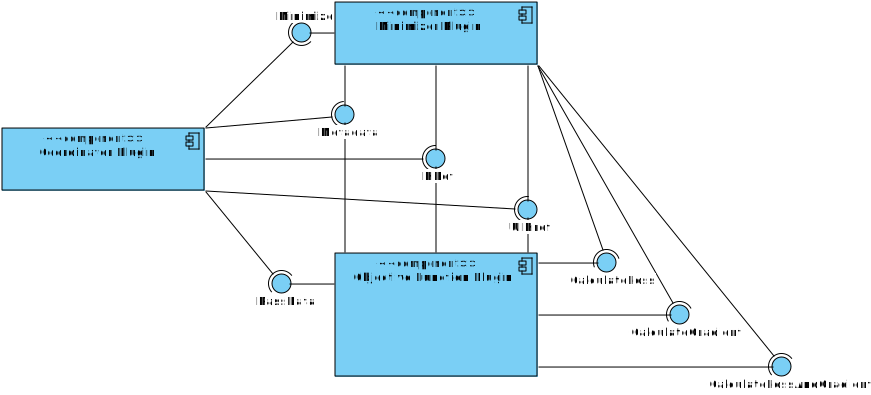
\includegraphics[width=\textwidth]{graphics/plugin_decomposition.svg}
    \caption{Component Diagram of decomposed optimization process}
    \label{fig:component_diagram}
\end{figure}

\subsection{Objective Function Plugin Interfaces}

The \gls{of} plugin interface is designed to accommodate a wide range of loss functions, including those that require gradient computation.
Its interfaces are:

\begin{itemize}
\item \textbf{Metadata}: The plugin provides metadata about itself as specified in the \gls{qhana} documentation \cite{Buehler2022}.
\item \textbf{UIRef}: This endpoint is used to obtain the microfrontend for the \gls{of} plugin, which is used to collect the hyperparameters from the user.
This interface also follows the \gls{qhana} documentation \cite{Buehler2022}.
\item \textbf{HRef}: This endpoint is used to process the input from the \gls{of} microfrontend and is therefore usually called the \textbf{processing} endpoint.
It is usually triggered by the user clicking the \emph{submit} button on the microfrontend.
This interface also follows the \gls{qhana} documentation \cite{Buehler2022}.
\item \textbf{PassData}: This endpoint is used to pass the input and target data to the \gls{of} plugin.
It returns the number of weights that are required for the optimization process.
The number of weights is returned here since it depends on the data and possibly the hyperparameters.
\item \textbf{CalculateLoss}: This endpoint calculates the loss.
\item \textbf{CalculateGradient (Optional)}: This endpoint is used to calculate the gradient of the loss function. It is optional since not all optimization algorithms require a gradient.
\item \textbf{CalculateLossAndGradient (Optional)}: This endpoint calculates the loss and the gradient of the loss function. Similar to the previous endpoint, it is optional since not all optimization algorithms require a gradient.
\end{itemize}

\subsection{Minimizer Plugin Interfaces}

The minimizer plugin, responsible for optimizing the loss function provided by the \gls{of} plugin, offers these interfaces:

\begin{itemize}
  \item \textbf{Metadata}: same as for the \gls{of} plugin
  \item \textbf{UIRef}: same as for the \gls{of} plugin
  \item \textbf{HRef}: same as for the \gls{of} plugin
  \item \textbf{Minimize}: This endpoint minimizes the loss function.
\end{itemize}

\subsection{Coordinator Plugin Interfaces}

The Coordinator plugin, orchestrating the interaction between the OF and Minimizer plugins, is equipped with the standard \gls{qhana} interfaces \textbf{Metadata}, \textbf{UIRef}, and \textbf{HRef}.

A systematic, consistent, and efficient optimization process is ensured by establishing these interfaces and ensuring that each plugin conforms to them.
This structured approach facilitates seamless interactions and fosters interchangeability, modularity, and extensibility, making it easy to add new \gls{of} and minimizer plugins in the future.

\section{Plugin Interaction Design}

The design of plugin interactions is pivotal to ensuring efficient and seamless coordination between different system components.
Given the extensive possibilities of interactions within the \gls{qhana} environment, the design phase was meticulous, considering various scenarios and ensuring adaptability.
The two primary modes of interactions were short-running and long-running, each catering to specific requirements.

\subsection{Short-Running Interaction}

In short-running interactions, a plugin invokes another plugin's endpoint, typically via a `GET` or a `Post` request, and immediately receives a response.
This mode of interaction is synchronous, wherein the invoking plugin waits for the response before proceeding.
Instances of such interactions in the optimization context are:
\begin{itemize}
    \item The coordinator plugin retrieves metadata from the \gls{of} and minimizer plugins.
    \item The coordinator plugin passes data to the \gls{of} plugin.
    \item The minimizer plugin calls the \texttt{CalculateLoss} endpoint of the \gls{of} plugin.
\end{itemize}

\subsubsection{Long-Running Interaction}

Long-running interactions come into play for processes that demand extensive computation time or involve multiple steps.
In such a case, the calling plugin invokes the endpoint of the invocable plugin.
The invoked endpoint then schedules a long-running task and returns immediately.
The calling plugin can then continue with its execution without waiting for the long-running task to finish.
A new endpoint for the calling plugin is defined that can be called by the long-running task once it is finished.
This endpoint is called a callback endpoint.
Instances of such interactions are:
\begin{itemize}
    \item The coordinator schedules the microfrontend of the \gls{of} plugin.
    The coordinator plugin provides a callback endpoint to the \gls{of} plugin that is called once the user enters the input and the input is processed.
    \item The coordinator schedules the microfrontend of the minimizer plugin.
    This mechanism works identically to the previous item.
    \item The coordinator plugin calls the minimization endpoint of the minimizer plugin.
    The minimizer plugin schedules the minimization process and returns immediately.
    Once the minimization process is finished, the minimizer plugin calls a callback endpoint of the coordinator plugin.
\end{itemize}
The design of these interactions ensures that plugins can interact seamlessly and efficiently regardless of the complexity or duration of tasks.

\section{Introduction of Interaction Endpoints}
\label{sec:introie}

Building upon the idea of plugins interacting with each other, as detailed in the previous section, there arises a crucial question:
How does one plugin discover the available endpoints of another?
This thesis introduces a novel concept called \textit{interaction endpoints} to \gls{qhana} to address this very challenge.

While \gls{qhana} already has a metadata field named "entry points," which are endpoints invoked by the \gls{qhana} UI to render a plugin's UI, interaction endpoints extend this idea further.
They specifically define endpoints in the metadata that other plugins can invoke, facilitating seamless integration and interaction.

The core of interaction endpoints is their \emph{type}.
All interaction endpoints with the same type must adhere to the same signature and return type.
This uniformity ensures that other plugins can interchangeably invoke them.
The \gls{of} plugin provides interaction endpoints of types \emph{calc\_loss}, \emph{calc\_grad}, \emph{calc\_loss\_and\_grad}, and \emph{of\_pass\_data}.
The minimizer plugin offers the `minimization' type.
These interaction endpoints correspond to the endpoints defined in the previous section.
The introduction of interaction endpoints significantly enhances the modularity and interchangeability within \gls{qhana}, paving the way for a more dynamic and adaptable plugin ecosystem.
More on how these interaction endpoints are implemented can be found in the implementation chapter \ref{chap: implementation}.

\section{Final Interaction Flow}
The architecture's final interaction flow can be broken down into three main parts, each ending in a new \gls{ui} displayed to the user.
They are visualized in the sequence diagrams in figures \ref{fig:interaction_flow_part1}, \ref{fig:interaction_flow_part2}, and \ref{fig:interaction_flow_part3}.

The first part begins after selecting the optimization plugin and concludes when the \gls{of} plugin's \gls{ui} is set as the next step.
Here, the coordinator plugin retrieves the user-selected \gls{of} and minimization plugin metadata, including their interaction endpoints.
This flow is represented in Figure \ref{fig:interaction_flow_part1}.

The second part starts with retrieving the \gls{of} plugin's microfrontend and ends when the minimizer plugin \gls{ui} is set as the next step.
After the user inputs hyperparameters and submits, the \gls{of} processes the input and sends a callback to the coordinator plugin,
The callback endpoint then passes the input and target data to the PassData endpoint.
This is depicted in Figure \ref{fig:interaction_flow_part2}.

The last segment starts with the minimizer plugin's microfrontend retrieval and ends when the optimization process concludes.
After users input the minimization hyperparameters, the minimizer processes the data and sends a callback to the coordinator.
The coordinator then triggers the minimization endpoint, initiating a long-running minimization task that continuously calls the \gls{of} calculation endpoint.
Once this task is completed, a final callback is made to the coordinator with the results.
This flow is shown in Figure \ref{fig:interaction_flow_part3}.

\begin{figure}[ht]
  \centering
  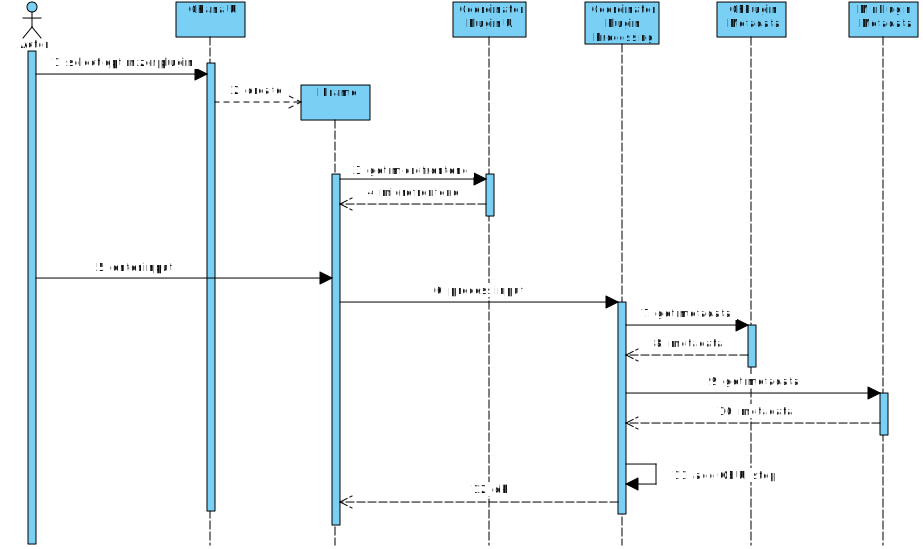
\includegraphics[width=\textwidth]{graphics/interaction_flow_1.svg}
  \caption{Final interaction flow of the first part of the optimization process.}
  \label{fig:interaction_flow_part1}
\end{figure}

\begin{figure}[ht]
  \centering
  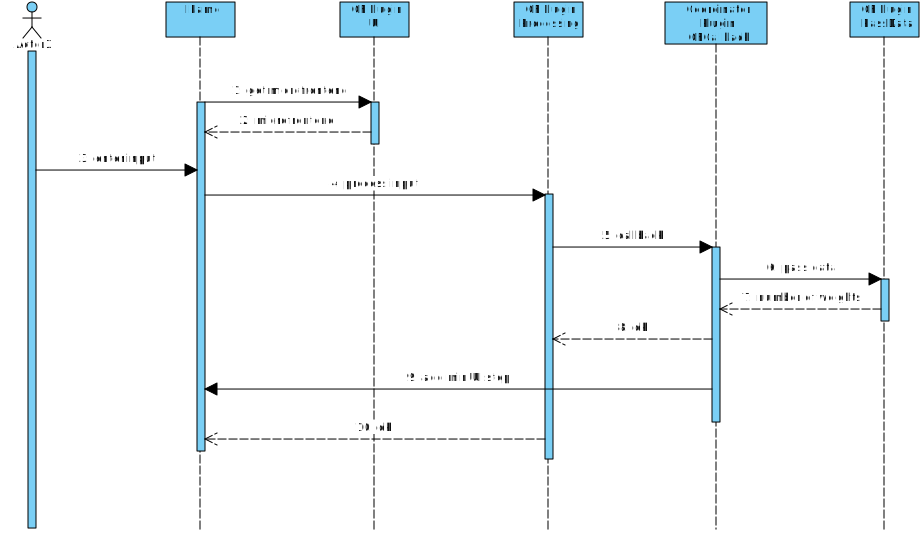
\includegraphics[width=\textwidth]{graphics/interaction_flow_2.svg}
  \caption{Final interaction flow of the second part of the optimization process.}
  \label{fig:interaction_flow_part2}
\end{figure}

\begin{figure}[ht]
  \centering
  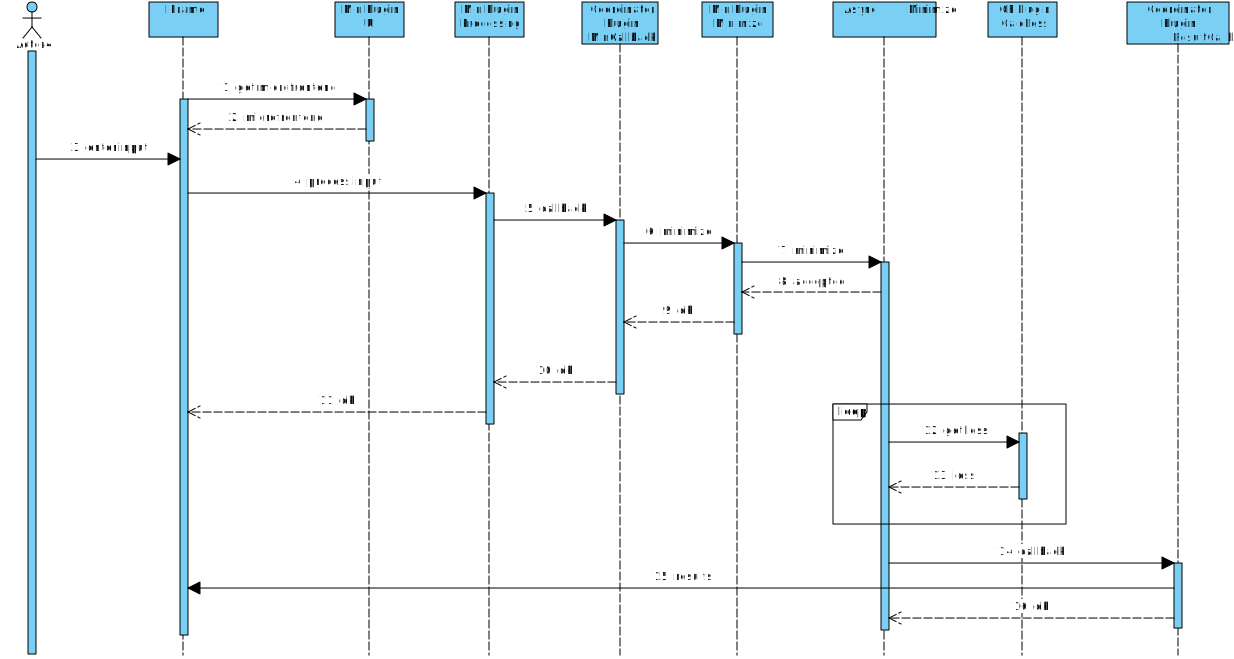
\includegraphics[width=\textwidth]{graphics/interaction_flow_3.svg}
  \caption{Final interaction flow of the third part of the optimization process.}
  \label{fig:interaction_flow_part3}
\end{figure}



\chapter{Implementation}
\label{chap:implementation}

The reader can find the resulting code that realized two different approaches to a plugin-based optimization framework in \gls{qhana} 's GitHub repository\footnote{\url{https://github.com/UST-QuAntiL/qhana-plugin-runner}}.
As examples, the code implements two types of minimizer plugins, the \emph{scipy-minimizer} and \emph{scipy-minimizer-grad} plugins, and three types of \gls{of} plugins, the \emph{ridge-loss}, \emph{hinge-loss}, and \emph{neural-network} plugins.
More on their implementation can be found in the following sections.
This chapter does not aim to provide a comprehensive overview of the code but to highlight the critical implementation details and differences between the two approaches.

\section{Directory Structure and Plugin Loading}
\label{sec:directoryStructure}

\gls{qhana} maintains two primary directories for plugin management: the \textit{plugins} and the \textit{stable plugins} directories.
The former contains plugins undergoing development, while the latter contains deployment-ready plugins.
Within these directories, individual plugins are neatly organized into dedicated subfolders.
Upon initiation, \gls{qhana} scans and loads plugins from these designated subfolders.

The focus of this thesis, the optimization plugin, resides in the \textit{plugins/optimization} directory.
Further divisions are made to promote clarity and a structured layout.

\begin{itemize}
  \item \textit{plugins/optimization/coordinator} – For the coordinator plugin.
  \item \textit{plugins/optimization/objective\_functions} – Where each \gls{of} plugin occupies its respective subfolder.
  \item \textit{plugins/optimization/minimizer} – Where each minimizer plugin occupies its respective subfolder.
\end{itemize}

Given that \gls{qhana}'s native architecture does not support the direct loading of plugins from nested subdirectories, a recursive plugin loader was developed for this purpose.
This loader traverses through the \textit{plugins} directory and its subdirectories.
The presence of an \textit{\_\_init\_\_.py} file within a folder confirms the plugin's legitimacy.
To exclude a plugin from the loading process, one places a \textit{.ignore} file in its respective folder.
The maximum recursion depth is limited to four to maintain system performance and a clear, structured layout.
This threshold sufficiently accommodates the current plugin structure but can be adjusted upwards if future needs arise.

The folder hierarchy is further enriched by including an \textit{interaction\_utils} directory dedicated to housing utility functions for generalized plugin interactions.
Additionally, there is a \textit{shared} directory, which stores data structures and schemas utilized across the plugins related to the optimization plugin.
A visual representation of the final folder structure, with all plugins implemented for this thesis, is shown in \cref{fig:folderStructure}.


\begin{figure}[h!]
  \dirtree{%
      .1 plugins.
      .2 optimizer.
      .3 coordinator.
      .3 interaction\_utils.
      .3 minimizer.
      .4 scipy\_minimizer.
      .4 scipy\_minimizer\_grad.
      .3 objective\_functions.
      .4 hinge\_loss.
      .4 neural\_network.
      .4 ridge\_loss.
      .3 shared.
  }
  \caption{QHana Plugin Folder Structure.}
  \label{fig:folderStructure}
\end{figure}

\section{Maintaining Context Across Plugin Endpoints}
\label{sec:contextBetweenPluginEndpoints}

The implementation leverages the multi-step plugin concept inherent to \gls{qhana} to preserve the continuity of information across different plugin endpoints.
In the \emph{processing} endpoint of a plugin, a database task is established, identifiable by a unique database ID.
This task stores all relevant context data, such as the hyperparameters designated for the minimization process.
Subsequent endpoints, like the \emph{minimization} endpoint, can access this stored context data by referencing the database task.
Notably, the endpoints' URL incorporates the database task's ID.


\section{UI Creation for Plugin Interaction}
\label{sec:uiCreationForPluginInteraction}
The QHAna platform provides a streamlined mechanism to craft simple \glspl{ui} with input fields generated from marshmallow schemas.
The primary step is to inherit from QHAna's \texttt{FrontendFormBaseSchema} class.
For the \gls{of} plugin, the input fields are the hyperparameters the loss function needs.
Listing \ref{lst:ridge_loss_schema} shows the \emph{ridge\-loss} plugin's hyperparameter, which is the regularization parameter \emph{alpha}.

\lstinputlisting[language=Python, caption={Ridge Loss Plugin Hyperparameter Schema.}, label=lst:ridge_loss_schema]{code/hyperparameter_schema_ridge.py}

The minimizer and \gls{of} plugin selection field is a critical input field for the coordinator plugin.
The \texttt{PluginUrl} class,  a custom class that extends marshmallow's \texttt{fields.Url} class generates that field.
It ensures that only plugins of the correct type are selected by checking a plugin's metadata for the correct label.
Imperative for this to work is that all minimizer plugins have the \emph{minimization} and all \gls{of} plugins have the \emph{objective-function} label.
Listing \ref{lst:coordinator_schema} shows the minimizer plugin selection field in the coordinator plugin's \gls{ui}.

\lstinputlisting[language=Python, caption=Coordinator Plugin UI Schema., label=lst:coordinator_schema]{code/ui_schema_coordinator.py}

As the \glspl{ui} of the \gls{of} and minimizer plugins are designed to be invoked by the coordinator plugin, the \emph{UIHref} which serves the \gls{ui} needs to accept a callback URL.
Therefore, all \emph{UIHref} endpoints of invocable plugins must include the \emph{CallbackUrlSchema} marshmallow schema as a query parameter.



\section{Invocation of Plugin Microfrontends by the Coordinator Plugin}
\label{sec:invocationOfPluginMicrofrontendsByTheCoordinatorPlugin}

As highlighted in the previous chapter, the coordinator plugin invokes the microfrontends of both the \gls{of} and minimizer plugins.
An adaptation of \gls{qhana}'s \emph{add\_step} function allows the invocation of a plugin's microfrontend by another plugin.
The \emph{add\_step} function's original purpose is to allow a multi-step plugin to show another of its microfrontends to the user.
The function was enhanced and renamed to \emph{invoke\_task}.
With this modification, the coordinator plugin can invoke another plugin's microfrontend by supplying the appropriate \emph{UIHref} and \emph{Href}.
Furthermore, the coordinator plugin can provide a callback URL to the invoked plugin.
This callback URL is a query parameter within the \emph{Href} and \emph{UIHref} URLs.

\section{Callback to the Coordinator Plugin}
\label{sec:implementationOfCallbacksToTheCoordinatorPlugin}

The coordinator plugin requires callbacks from invocable plugins in two distinct scenarios:
\begin{enumerate}
    \item After the user submits the microfrontend of either the minimization or the \gls{of} plugin.
    \item Once the asynchronous minimization process concludes.
\end{enumerate}

For the first scenario, the process unfolds as follows:
\begin{itemize}
    \item The coordinator invokes the microfrontend of the invocable plugin using the \emph{invoke\_task} function, as elaborated in Section \ref{sec:invocationOfPluginMicrofrontendsByTheCoordinatorPlugin}.
    \item On user submission of the microfrontend, the callback URL is passed to the processing endpoint of the invocable plugin via a query parameter.
    \item Subsequently, the invoked plugin makes a post request to the callback URL.
\end{itemize}

In contrast, the second scenario operates through the following mechanism:
\begin{itemize}
    \item The coordinator plugin initiates a post request to the minimizer plugin's minimization endpoint, embedding a callback URL within the body.
    \item The minimizer plugin schedules an asynchronous celery task for loss function minimization.
    It registers the callback URL in the database under the designation \emph{status\_changed\_callback\_urls}.
    This label is pivotal for subsequent retrieval of the callback URL.
    \item The endpoint returns, and the celery task commences the minimization process.
    \item Following the task's completion, its status updates through the already implemented \emph{save\_task\_result} function.
    This action now triggers a signal when it finishes or runs into an error, courtesy of Python's \emph{blinker} library, indicating the status change and passing the database ID of the task as an argument.
    \item A dedicated signal handler retrieves the callback and task view URL from the database.
    The handler then orchestrates a post request to the callback URL, embedding the task view URL within the body.
\end{itemize}
Listing \ref{lst:signal_handler} presents the implementation of the signal handler, while Listing \ref{lst:singal_emitter} illustrates the juncture where the signal is emitted.

\lstinputlisting[language=Python, caption=Signal Handler for Callbacks., label=lst:signal_handler]{code/signal_handler.py}
\lstinputlisting[language=Python, caption=Signal Emitter for Callbacks., label=lst:singal_emitter]{code/signal_emitter.py}


\section{Implementation of Interaction Endpoints}
\label{sec:implementationOfInteractionEndpoints}

The essence of the plugin-based optimization framework lies in its interaction endpoints.
These endpoints standardize the interchangeability of inputs and outputs.
Marshmallow schemas are the backbone of the implementation to manage this standardized data exchange.

\subsection{Interaction Endpoint Schemas}
The repository's shared folder contains the defined schemas.
Each interaction endpoint type has an associated input and output schema.
If a plugin wishes to invoke another plugin's interaction endpoint, it can populate the input schema and parse the response using the output schema.
In the implementation, the \gls{of} plugin defines schemas for the following interaction endpoints:
\begin{itemize}
  \item \textbf{pass\_data}: Uses \emph{ObjectiveFunctionPassDataSchema} for input and \emph{ObjectiveFunctionPassDataResponseSchema} for output.
  \item \textbf{calc\_loss}: Uses \emph{CalcLossOrGradInputSchema} for input and \emph{LossResponseSchema} for output.
\end{itemize}
For the minimizers' \emph{minimization} endpoint, the input schema is \emph{MinimizerInputSchema}.
The output, meanwhile, is a simple 200 status code, signaling the initiation of the minimization process.
Another implementation challenge revolves around ensuring that plugins can discover the endpoints of other plugins, which is solved in section \ref{sec:metadataEndpoint}, but first section
\ref{sec:customMarshmallowFieldForData} introduces a custom marshmallow field for input and target data.

\subsection{Custom Marshmallow Field for Data}
\label{sec:customMarshmallowFieldForData}
To streamline the input and target data exchange between plugins, a custom marshmallow field, \emph{NumpyArray}, was introduced (see \ref{lst:numpy_array_schema}).
Specifically crafted to handle NumPy arrays, this versatile field can accommodate arrays of any dimensionality with JSON-serializable data types.
It aids in data transfer between endpoints and ensures efficient data storage in the database.
\lstinputlisting[language=Python, caption=Custom Marshmallow Field for NumPy Arrays., label=lst:numpy_array_schema]{code/numpy_array_schema.py}

\subsection{Metadata Endpoint and Interaction Endpoint Discovery}
\label{sec:metadataEndpoint}
The metadata of plugins houses the definitions for interaction endpoints.
Traditionally, the \emph{EntryPoint} field in the metadata was reserved for guiding the \gls{qhana} UI to a plugin's microfrontend.
However, this thesis expands the \emph{EntryPoint} field to encompass interaction endpoints.
The \emph{interactionEndpoints} field is essentially a list, potentially containing multiple interaction endpoints.
Each list entry is a dictionary containing a \textbf{type} and an \textbf{href} field.
The \textbf{type} field, a string, denotes the endpoint type.
It is made user-friendly by providing the \emph{InteractionEndpointType} enum in the shared folder, which lists all possible endpoint types for the optimization process.
The \textbf{href} field houses the endpoint's URL.
Listing \ref{lst:metadata} illustrates this using the \emph{ridge-loss} plugin's metadata.

\lstinputlisting[language=Python, caption=Metadata of the Ridge Loss Plugin., label=lst:metadata]{code/metadata.py}

For multi-step plugins, the interaction endpoint's definition in metadata slightly deviates.
As discussed in \ref{sec:contextBetweenPluginEndpoints}, multi-step plugins incorporate a runtime-specific database ID into the URL.
The \emph{href} field functions as a format string that allows the substitution of a placeholder with the actual database ID.
Listing \ref{lst:metadata_multistep} offers a glimpse into this, showcasing the \emph{ridge-loss} plugin implemented as a multi-step entity.
The invoking plugin replaces the placeholder with the actual database ID when known.
This distinction is foundational to the differences between the two approaches, explored further in the subsequent section.
\lstinputlisting[language=Python, caption=Metadata of the Ridge Loss Plugin as a Multi-Step Plugin., label=lst:metadata_multistep]{code/metadata_multistep.py}


\section{Exemplary Minimizers and Objective Functions}
\label{sec:exampleMinimizersAndObjectiveFunctions}

The implementation encompassed two distinct minimizer plugins and three \gls{of} plugins to illustrate the capabilities of the plugin-based optimization framework.
Specifically, the minimizer plugins \emph{scipy-minimizer} and \emph{scipy-minimizer-grad} and the \gls{of} plugins \emph{ridge-loss}, \emph{hinge-loss}, and \emph{neural-network}.

\subsection{Minimizer Plugins}
\label{sec:minimizerPlugins}

At the core, both plugins use \emph{scipy.optimize.minimize} as their minimization algorithm.
The \emph{scipy-minimizer} plugin leverages this method to minimize the loss function without needing a gradient.
Its sole input hyperparameter is the minimization method, restricted to methods that operate without a gradient.

On the other hand, the \emph{scipy-minimizer-grad} plugin employs the same method but incorporates the gradient for loss minimization.
It accepts input hyperparameters that exclusively pertain to methods necessitating the gradient.
Regardless of their approach, both plugins yield the weights that optimize the loss function's minimization.

\subsection{Objective Function Plugins}
\label{sec:objectiveFunctionPlugins}

The \emph{ridge-loss} plugin encapsulates the ridge loss function, as depicted in \ref{alg:ridge_loss}.
It operates with the regularization parameter \emph{alpha} as its input hyperparameter.
In a similar vein, the \emph{hinge-loss} plugin embodies the hinge loss function, showcased in \ref{alg:hinge_loss}, and uses the regularization parameter \emph{C} as its input.

The \emph{neural-network} plugin employs a neural network featuring a single hidden layer.
Its hyperparameters include the count of neurons present in this hidden layer.
Notably, this plugin facilitates the gradient calculation for the loss function, making it compatible with the \emph{scipy-minimizer-grad} plugin.
The user is highly encouraged to refer to the code repository for a more in-depth understanding of how a more sophisticated method is implemented for loss calculation.


\begin{lstlisting}[caption={Ridge Loss Calculation}, label=alg:ridge_loss]
  def ridge_loss(X, w, y, alpha):
      # Calculate the predicted values using the weight vector
      y_pred = X.dot(w)

      # Compute the mean squared error between actual and predicted values
      mse = mean((y - y_pred) ** 2)

      # Calculate the ridge penalty using the weight vector
      ridge_penalty = alpha * sum(w**2)

      # Combine the mean squared error and ridge penalty to get the total ridge loss
      total_loss = mse + ridge_penalty

      return total_loss
\end{lstlisting}

\begin{lstlisting}[caption={Hinge Loss Calculation}, label=alg:hinge_loss]
  def hinge_loss(X, w, y, C):
      # Get the number of samples from the input matrix
      n_samples, _ = X.shape

      # Initialize the loss to zero
      loss = 0.0

      # Iterate over each sample in the dataset
      for i in range(n_samples):
          # Calculate the score for the current sample using the weight vector
          score = np.dot(w, X[i])

          # Compute the hinge loss for the current sample and accumulate
          loss += max(0, 1 - y[i] * score)

      # Apply the regularization term to the accumulated loss
      loss = C * loss / n_samples

      # Add the l2 regularization term to the loss
      loss += 0.5 * np.dot(w, w)

      return loss
\end{lstlisting}

\section{Comparative Analysis of Plugin-Based Implementation Strategies}
\label{sec:differencesBetweenTheTwoPluginBasedImplementationApproaches}

The implementation resulted in two distinct methodologies for constructing a plugin-based optimization framework.
This section outlines the intrinsic differences that characterize each strategy.

\subsection{Decoupled Plugin Approach}
\label{sec:firstApproach}

The foundational idea behind the first approach is promoting maximal decoupling between plugins, which particularly applies to the \gls{of} plugin.
This idea entails minimizing data transfer between plugins and emphasizing data retrieval directly from the database whenever feasible.

Specifically, the \gls{of} plugin archives its hyperparameters in the database.
When the \emph{pass\_data} endpoint is invoked, input and target data get stored in the database.
Thus, for the \emph{pass\_data} endpoint, which determines the number of input weights, the coordinator plugin only passes the input and target data since the \gls{of} plugin fetches the hyperparameters from the database.
The loss calculation endpoints \emph{calc\_loss}, \emph{calc\_grad}, and \emph{calc\_loss\_and\_grad} solely need the weights as input, leveraging already stored hyperparameters and data.
Listing \ref{lst:calc_loss_schema} illustrates an exemplary schema for the \emph{calc\_loss} endpoint.

Consequently, for the minimizer plugin, there is no occasion where knowledge of the \gls{of} 's hyperparameters or its data is essential, leading to a lean input schema for the \emph{minimization} endpoint, as depicted in Listing \ref{lst:minimization_schema}.
However, it mandates that the task's database ID be communicated to the coordinator plugin through the microfrontend callback process, essential for managing interaction endpoint URLs, as discussed in \ref{sec:metadataEndpoint}.

\subsection{Integrated Plugin Approach}
\label{sec:secondApproach}

The second strategy embodies a tighter integration.
This approach does not implement the \gls{of} plugin as a multi-step plugin.
Such an implementation implies that no shared context exists among the plugin's endpoints, necessitating the passing of all required data during each endpoint invocation.

This requires the microfrontend callback process to relay the hyperparameters to the coordinator plugin.
The coordinator then transmits the hyperparameters and data to the \gls{of} plugin's \emph{pass\_data} endpoint.
In this setup, the minimizer plugin must also store the hyperparameters and data since it must relay this to the \gls{of} plugin's loss calculation endpoint.
Listing \ref{lst:calc_loss_schema_multistep} exhibits the input schema for the \emph{calc\_loss} endpoint, while Listing \ref{lst:minimization_schema_multistep} demonstrates the \emph{minimization} endpoint's schema.
Passing the hyperparameters of a \gls{of} plugin ensures that neither the coordinator nor the minimizer plugin requires in-depth knowledge of the hyperparameters irrespective of the \gls{of} 's internal mechanics.
As a trade-off, there is no need to relay a task's database ID to the coordinator.

\chapter{Results}
\label{chap:results}
In this Chapter the results that can be achieved with the inplmenentation in place are presented.
The resutls this chapter focuses on are the performance of the system, the interchangeability of plugins, and the usability for developers.

\section{Performance Analysis}
\label{sec:performanceAnalysis}

In this section the performance of the system is measured as described in section \ref{subsec:performanceBenchmarking} and the results are presented.

\subsection{Hardware and System Specifications}
\label{subsec:hardwareAndSystemSpecifications}

The benchmarks were conducted on a MacBook Pro. The detailed specifications of the machine are as follows:

\begin{itemize}
    \item \textbf{Model:} MacBookPro18,1
    \item \textbf{Processor (CPU):} Apple M1 Pro
    \item \textbf{Memory (RAM):} 32 GB (hw.memsize: 34359738368 bytes)
    \item \textbf{Graphics Processing Unit (GPU):}
    \begin{itemize}
        \item Chipset Model: Apple M1 Pro
        \item Type: GPU
        \item Bus: Built-In
        \item Total Number of Cores: 16
        \item Metal Support: Metal 3
    \end{itemize}
    \item \textbf{Operating System:} macOS, Version 13.4.1, Build Version: 22F770820d
\end{itemize}

\subsection{Benchmarking Results}
\label{subsec:benchmarkingResults}

The most time consuming part of the minimization process is the calculation of the loss function, since it is called several times during the minimization process.
For the benchmarking the \emph{ridge-loss} plugin is used as the \gls{of} with \emph{alpha} set to 0.5 and the \emph{scipy-minimizer} plugin is used as the minimizer with the \emph{method} set to \emph{L-BFGS-B}.

Table \ref{table:of_calls} shows how often the loss is evaluated during the minimization process across different datasets, underlying the importance of the performance of the loss function calculation.


\begin{table}[h!]
  \centering
  \begin{tabular}{cc}
  \toprule
  \textbf{Number of Data Points} & \textbf{Number of Evaluations} \\
  \midrule
  200 & 264 \\
  400 & 341 \\
  600 & 370 \\
  800 & 430 \\
  1000 & 480 \\
  1200 & 520 \\
  1400 & 570 \\
  \bottomrule
  \end{tabular}
  \caption{Number of times the loss function is evaluated during minimization across different dataset sizes.}
  \label{table:of_calls}
\end{table}

Figure \ref{fig:of_call_time_version1} shows the time it takes for a single call of the loss function for different dataset sizes for the first plugin-based implementation approach.
The \emph{Calculation Time} captures only the actual time it takes to calculate ridge loss.
The \emph{Database Time} measures the time it takes to retrieve the data from the database.
The \emph{Network Time} measures the time it takes to send the data to the \gls{of} plugin and receive the result.
The total time it takes from the point at which the minimizer plugin calls the calculation endpoint until it receives the result is the sum of the \emph{Calculation Time}, \emph{Database Time}, and \emph{Network Time}.

\begin{figure}
  \centering
  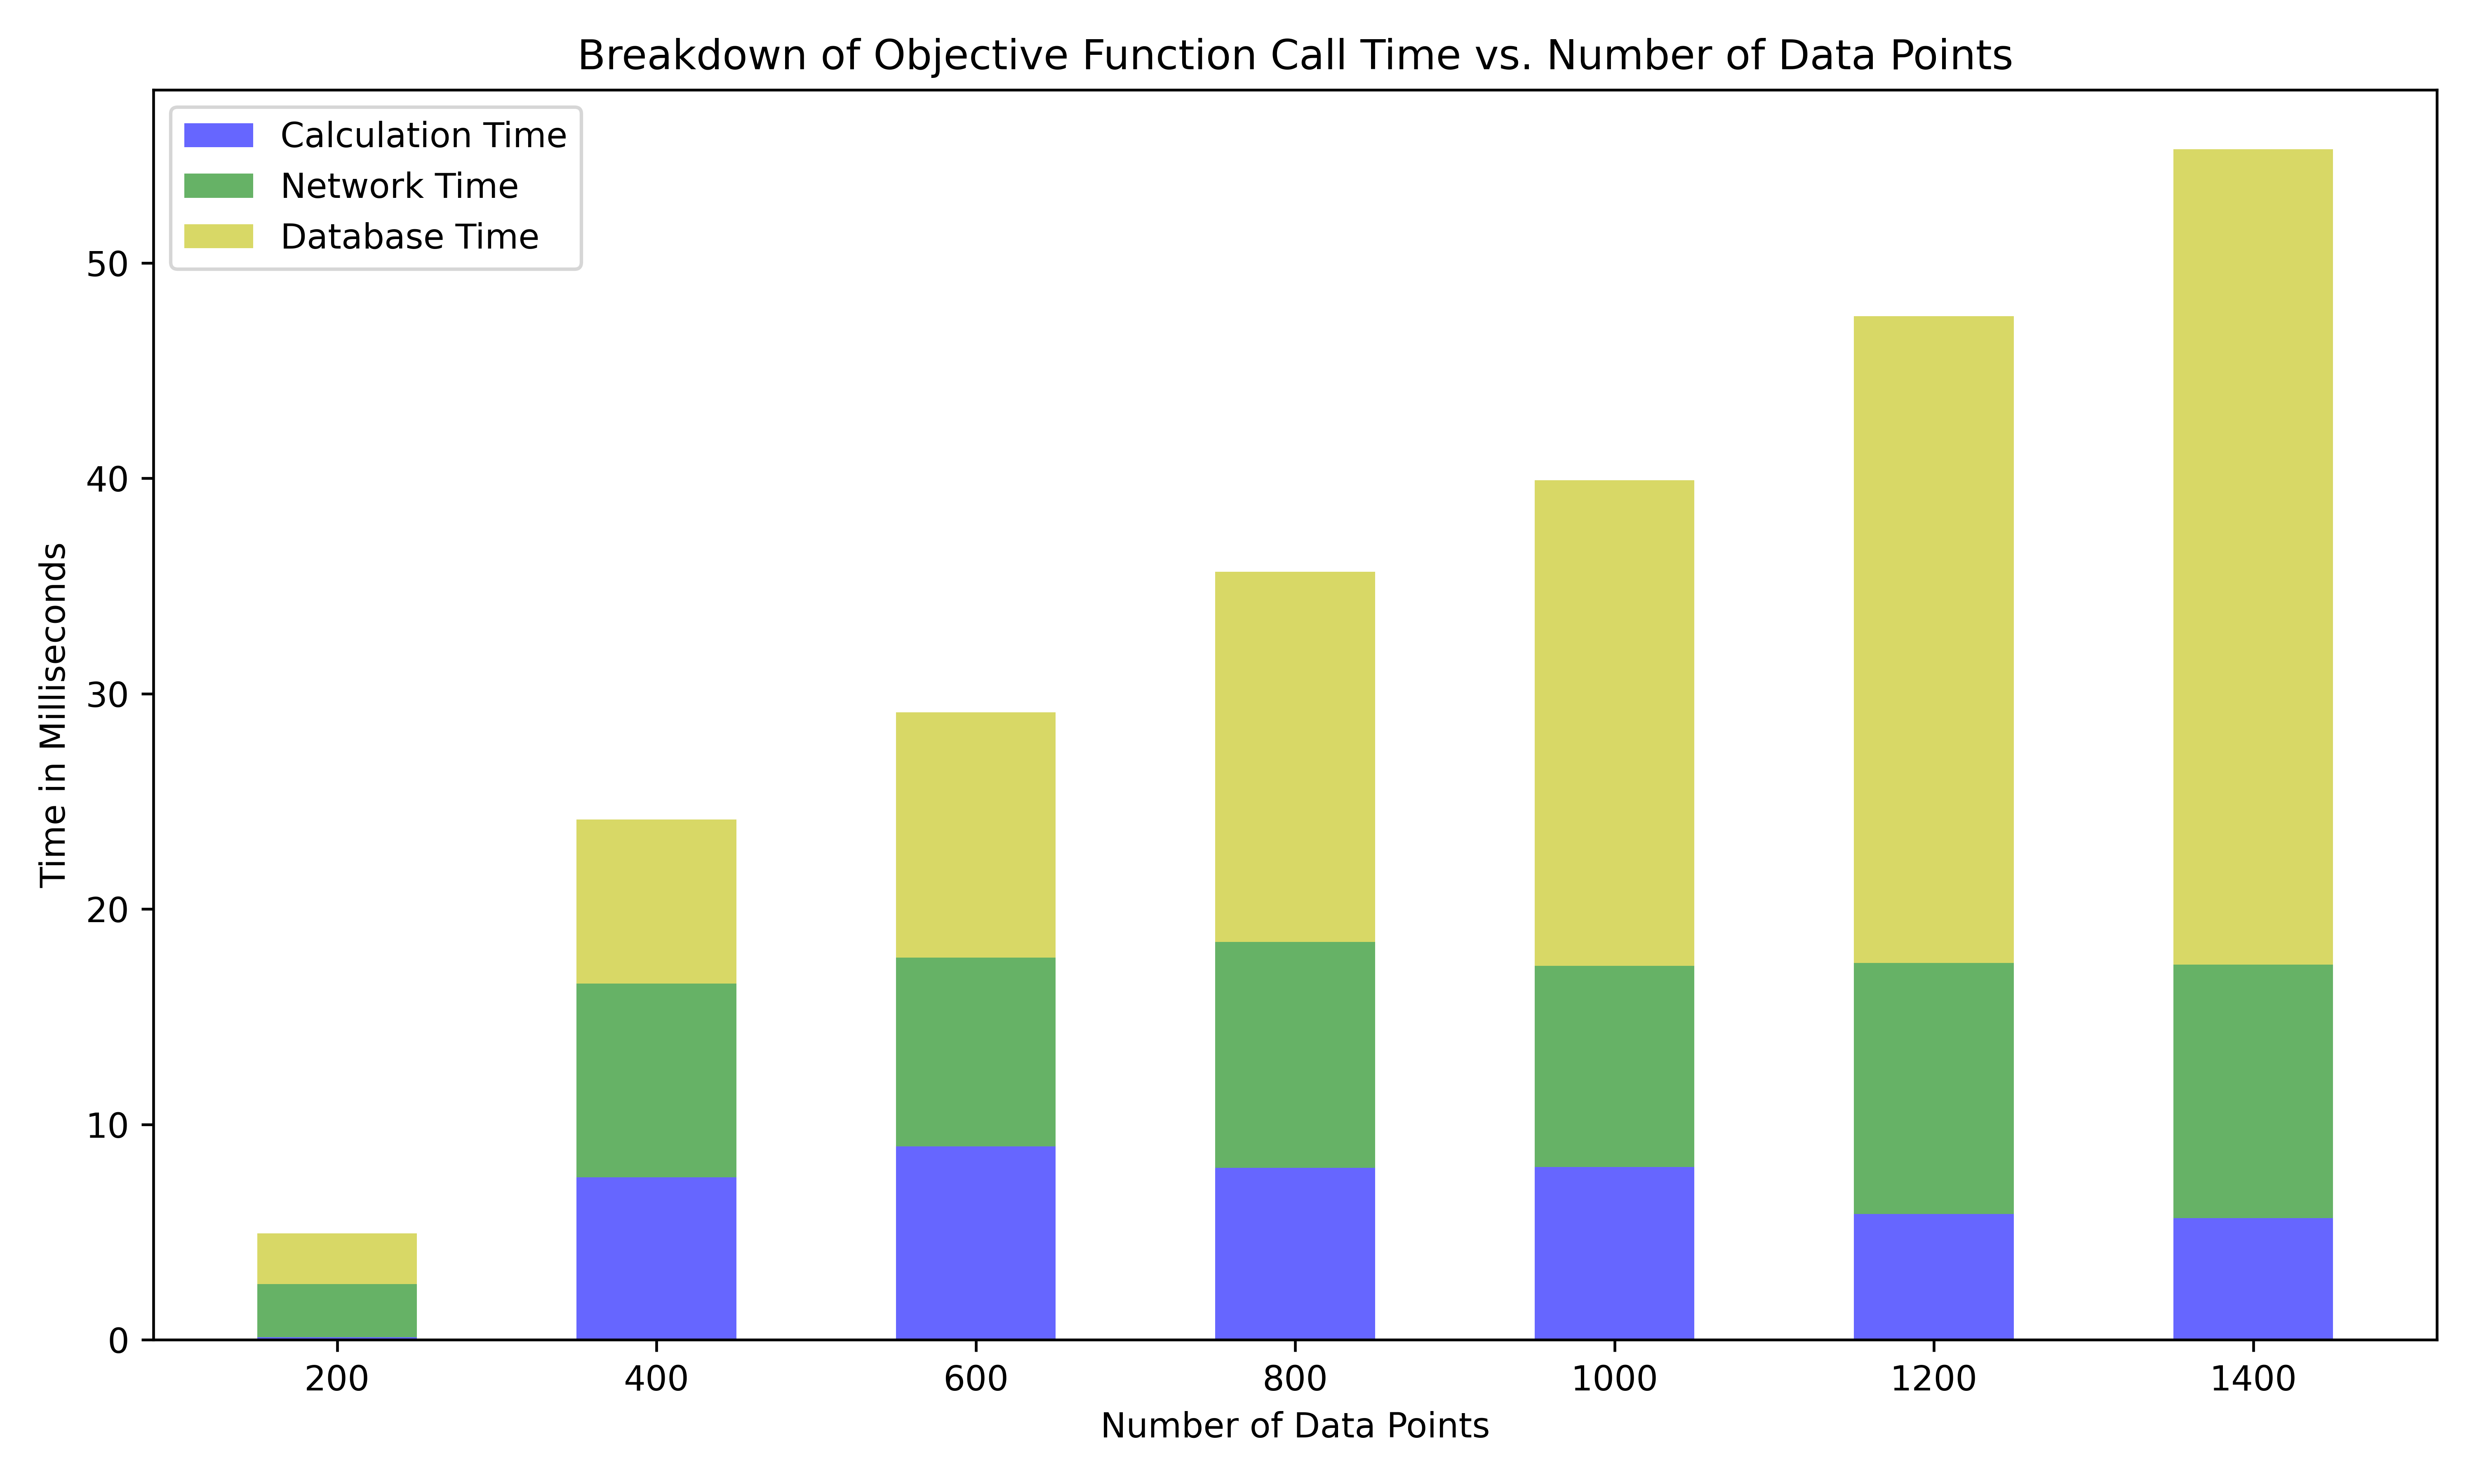
\includegraphics[width=\textwidth]{graphics/of_call_times_version1.png}
  \caption{Time it takes for a single call to the \emph{calc\_loss} endpoint of the \emph{ridge-loss} plugin for different dataset sizes for the first plugin-based implementation approach.}
  \label{fig:of_call_time_version1}
\end{figure}

Figure \ref{fig:of_call_time_version2} caputes the same measurements for the second plugin-based implementation approach.
Since the \gls{of} plugin is not implemented as a multi-step plugin, the \emph{Database Time} is not measured.

\begin{figure}
  \centering
  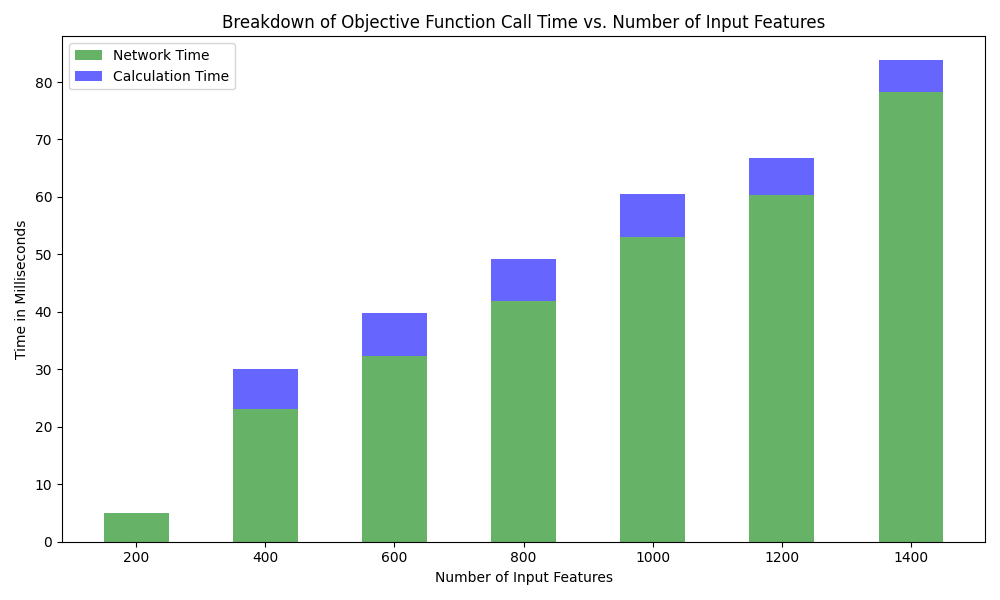
\includegraphics[width=\textwidth]{graphics/of_call_times_version2.png}
  \caption{Time it takes for a single call to the \emph{calc\_loss} endpoint of the \emph{ridge-loss} plugin for different dataset sizes for the second plugin-based implementation approach.}
  \label{fig:of_call_time_version2}
\end{figure}

Figure \ref{fig:coparison_of_of} shows a comparison between the total times it takes to calcualte the loss function across different implementations including the jupyter notebook based implementation.

\begin{figure}
  \centering
  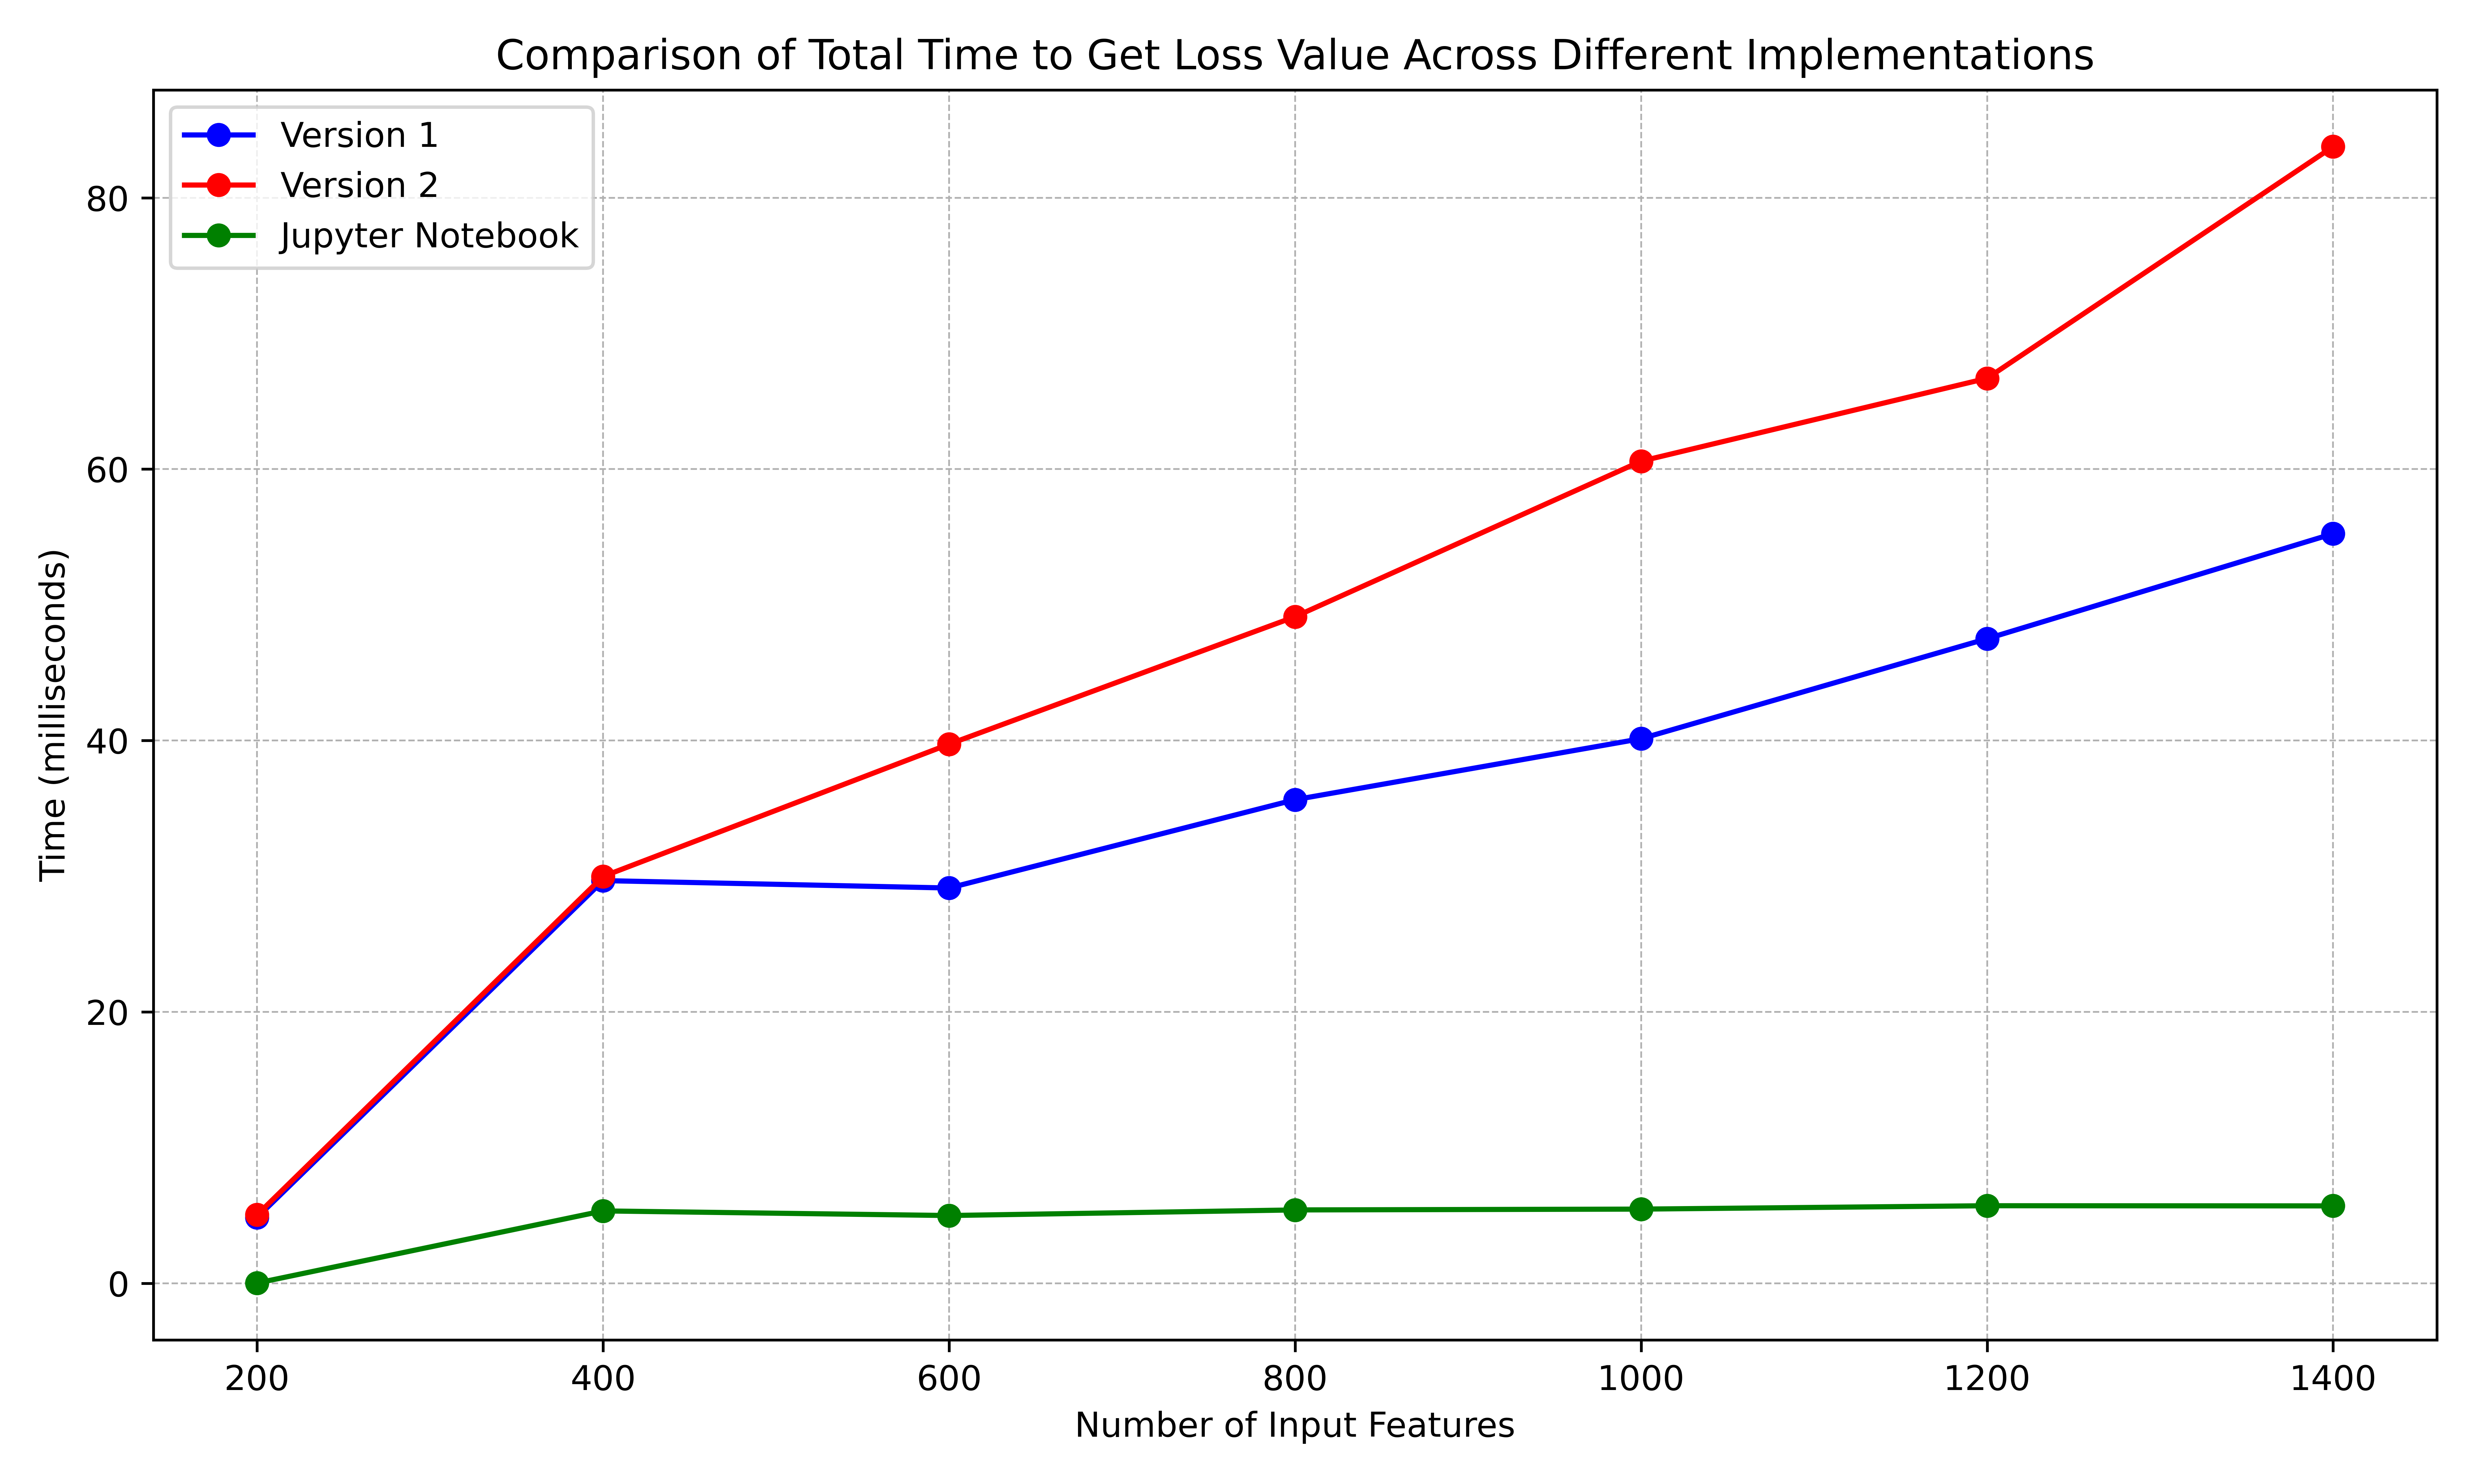
\includegraphics[width=\textwidth]{graphics/comparison_of_of.png}
  \caption{Comparison of the total time it takes to get the loss value across different implementations including the jupyter notebook based implementation.}
  \label{fig:coparison_of_of}
\end{figure}

Figure \ref{fig:time_for_of_calc} measures the same metrics as Figure \ref{fig:coparison_of_of} but this time it ignores the \emph{Database Time} and the \emph{Network Time} only measuring the actual \emph{Calculation Time}.

\begin{figure}
  \centering
  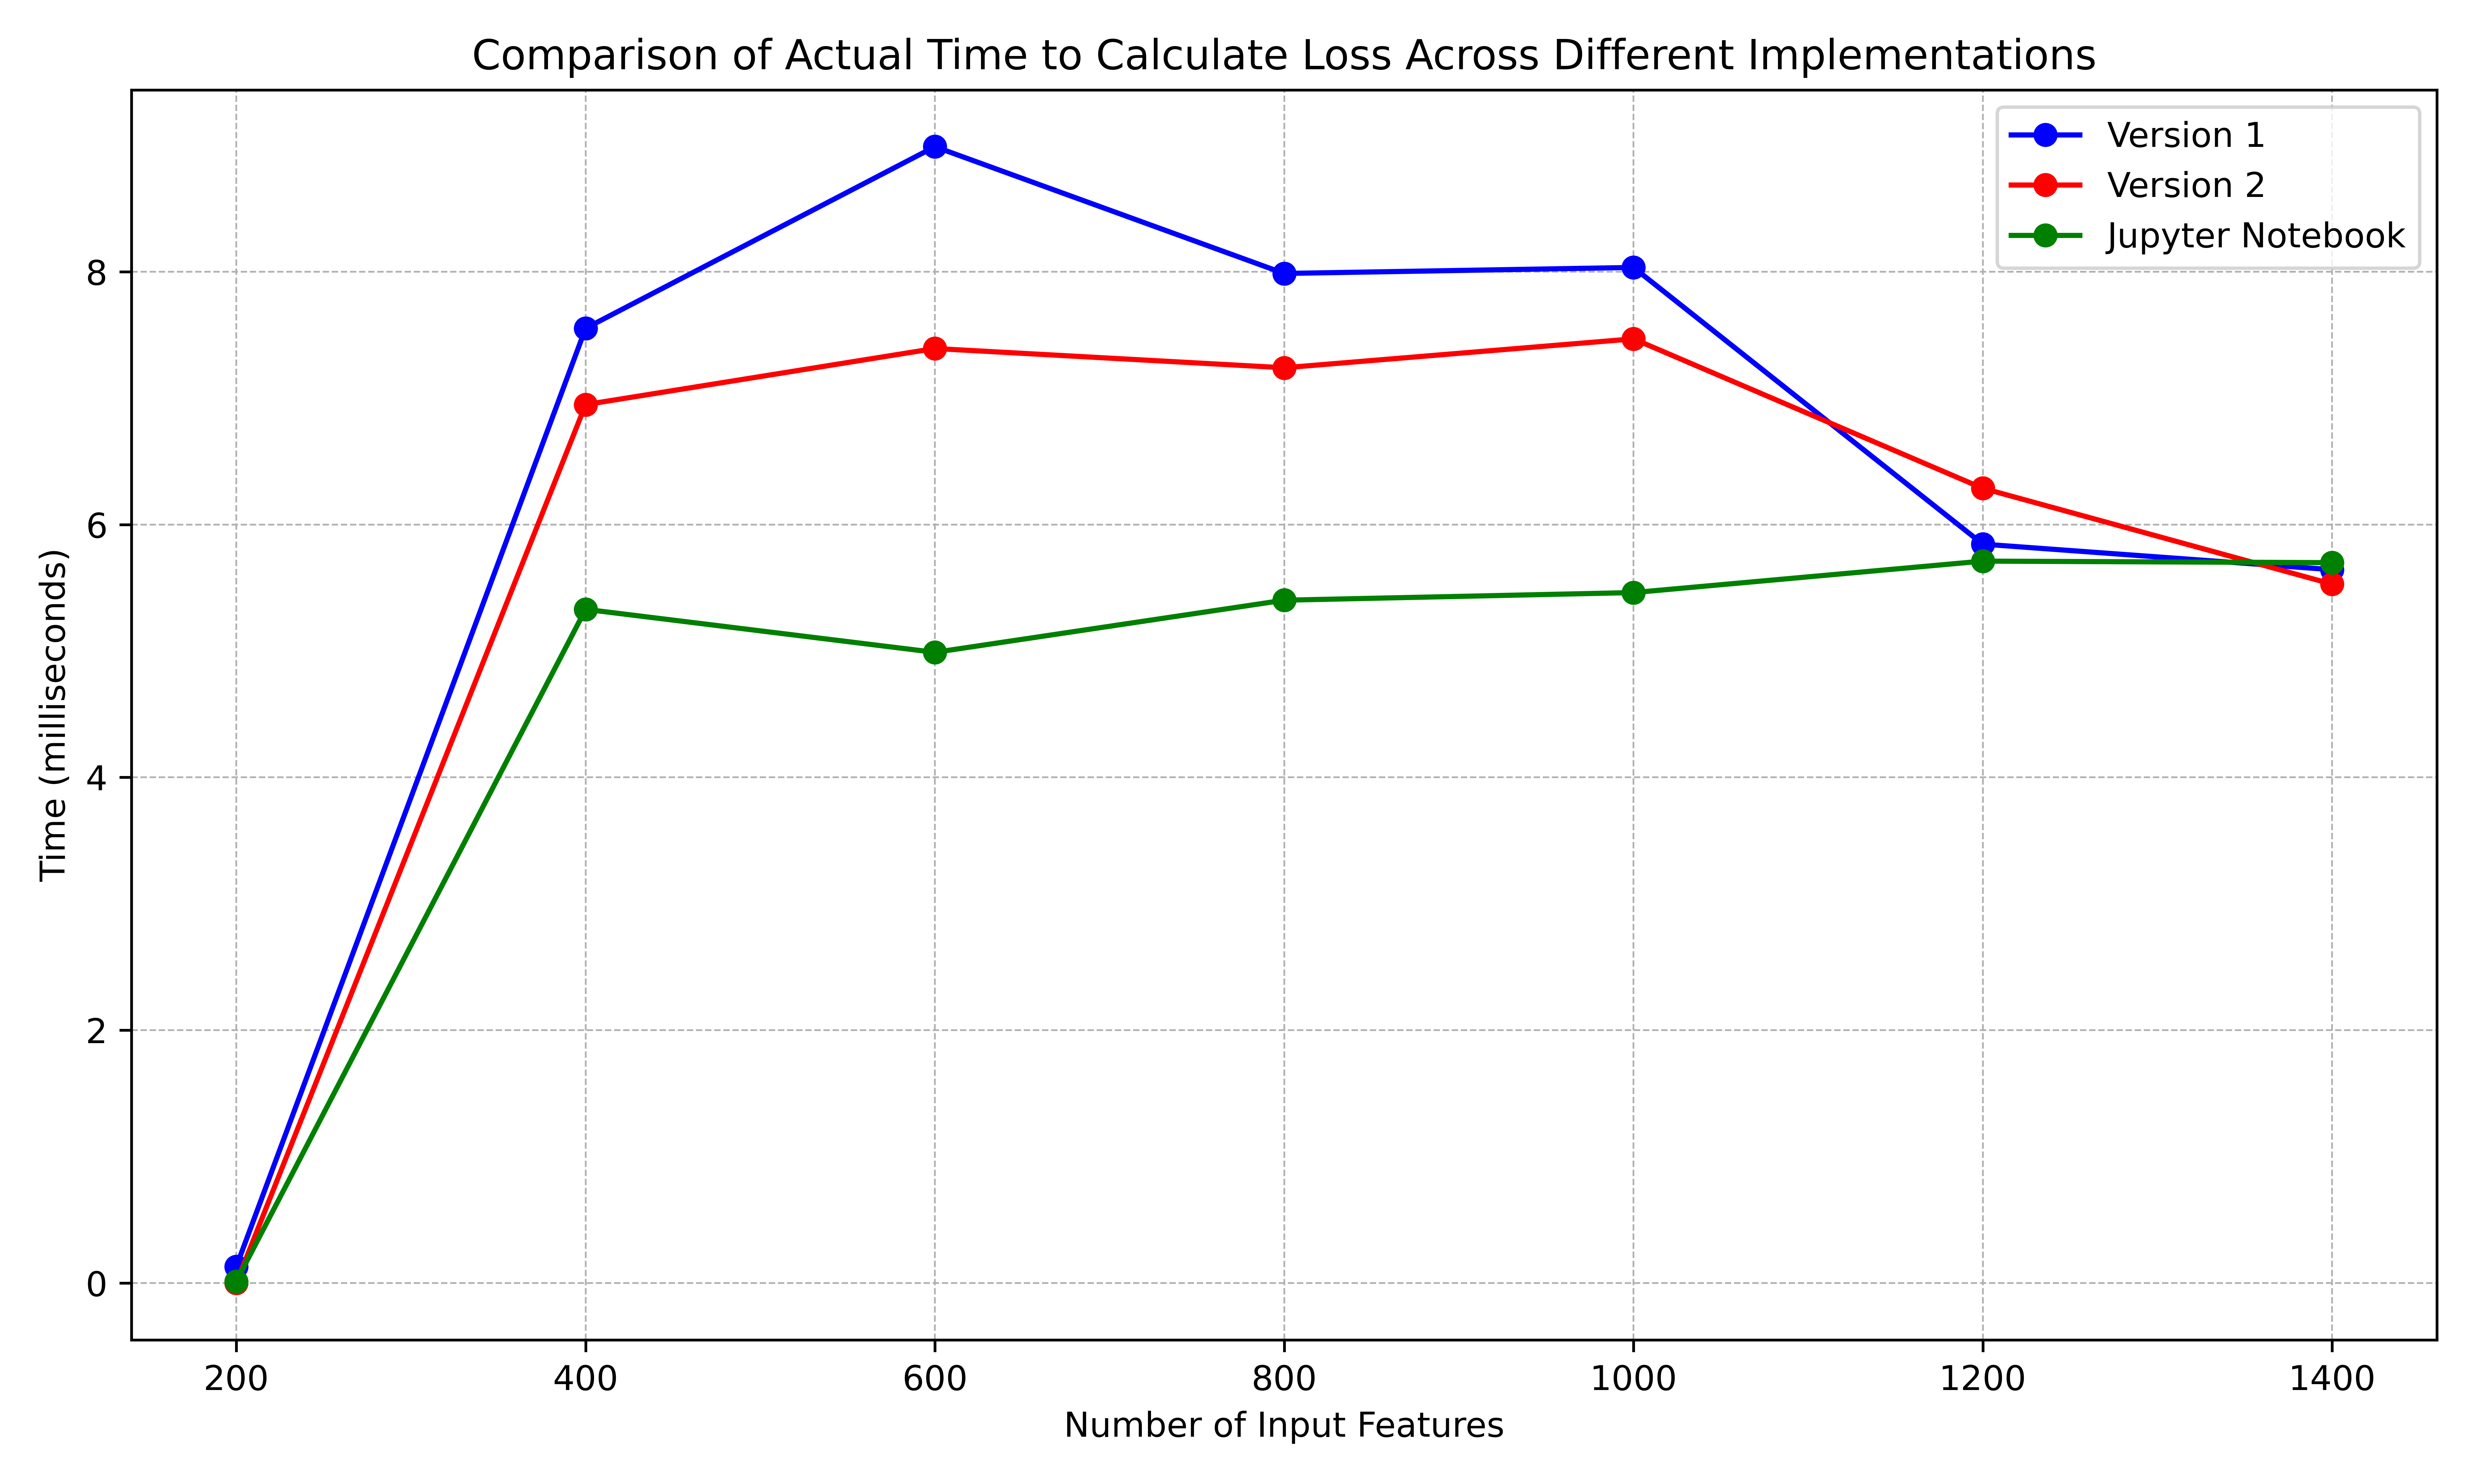
\includegraphics[width=\textwidth]{graphics/time_for_of_calc.png}
  \caption{Comparison of the time the actual loss calculation takes across different implementations including the jupyter notebook based implementation.}
  \label{fig:time_for_of_calc}
\end{figure}

Obviously one can see that the jupyter notebook based implementation is the fastest, since it does not have to deal with network latency.
Especially for the first plugin-based implementation approach the database latency is a bottleneck, that can be avoided.

% \subsection{Caching of Data}
% \label{subsec:cachingOfData}

% In order to avoid the database latency, a caching mechanism is implemented for the first plugin-based implementation approach.
% Since the input and target data and the hyperparameters do not change during the minimization process, they can be cached.
% That means during the first call of the \emph{calc\_loss} endpoint the data is retrieved from the database and cached for subsequent calls.
% For the implementation the \emph{flask-caching} library is used.
% Figure \ref{fig:of_call_time_version1_cached} compares the loss calculation time for the first plugin-based implementation approach with and without caching.

% \begin{figure}
%   \centering
%   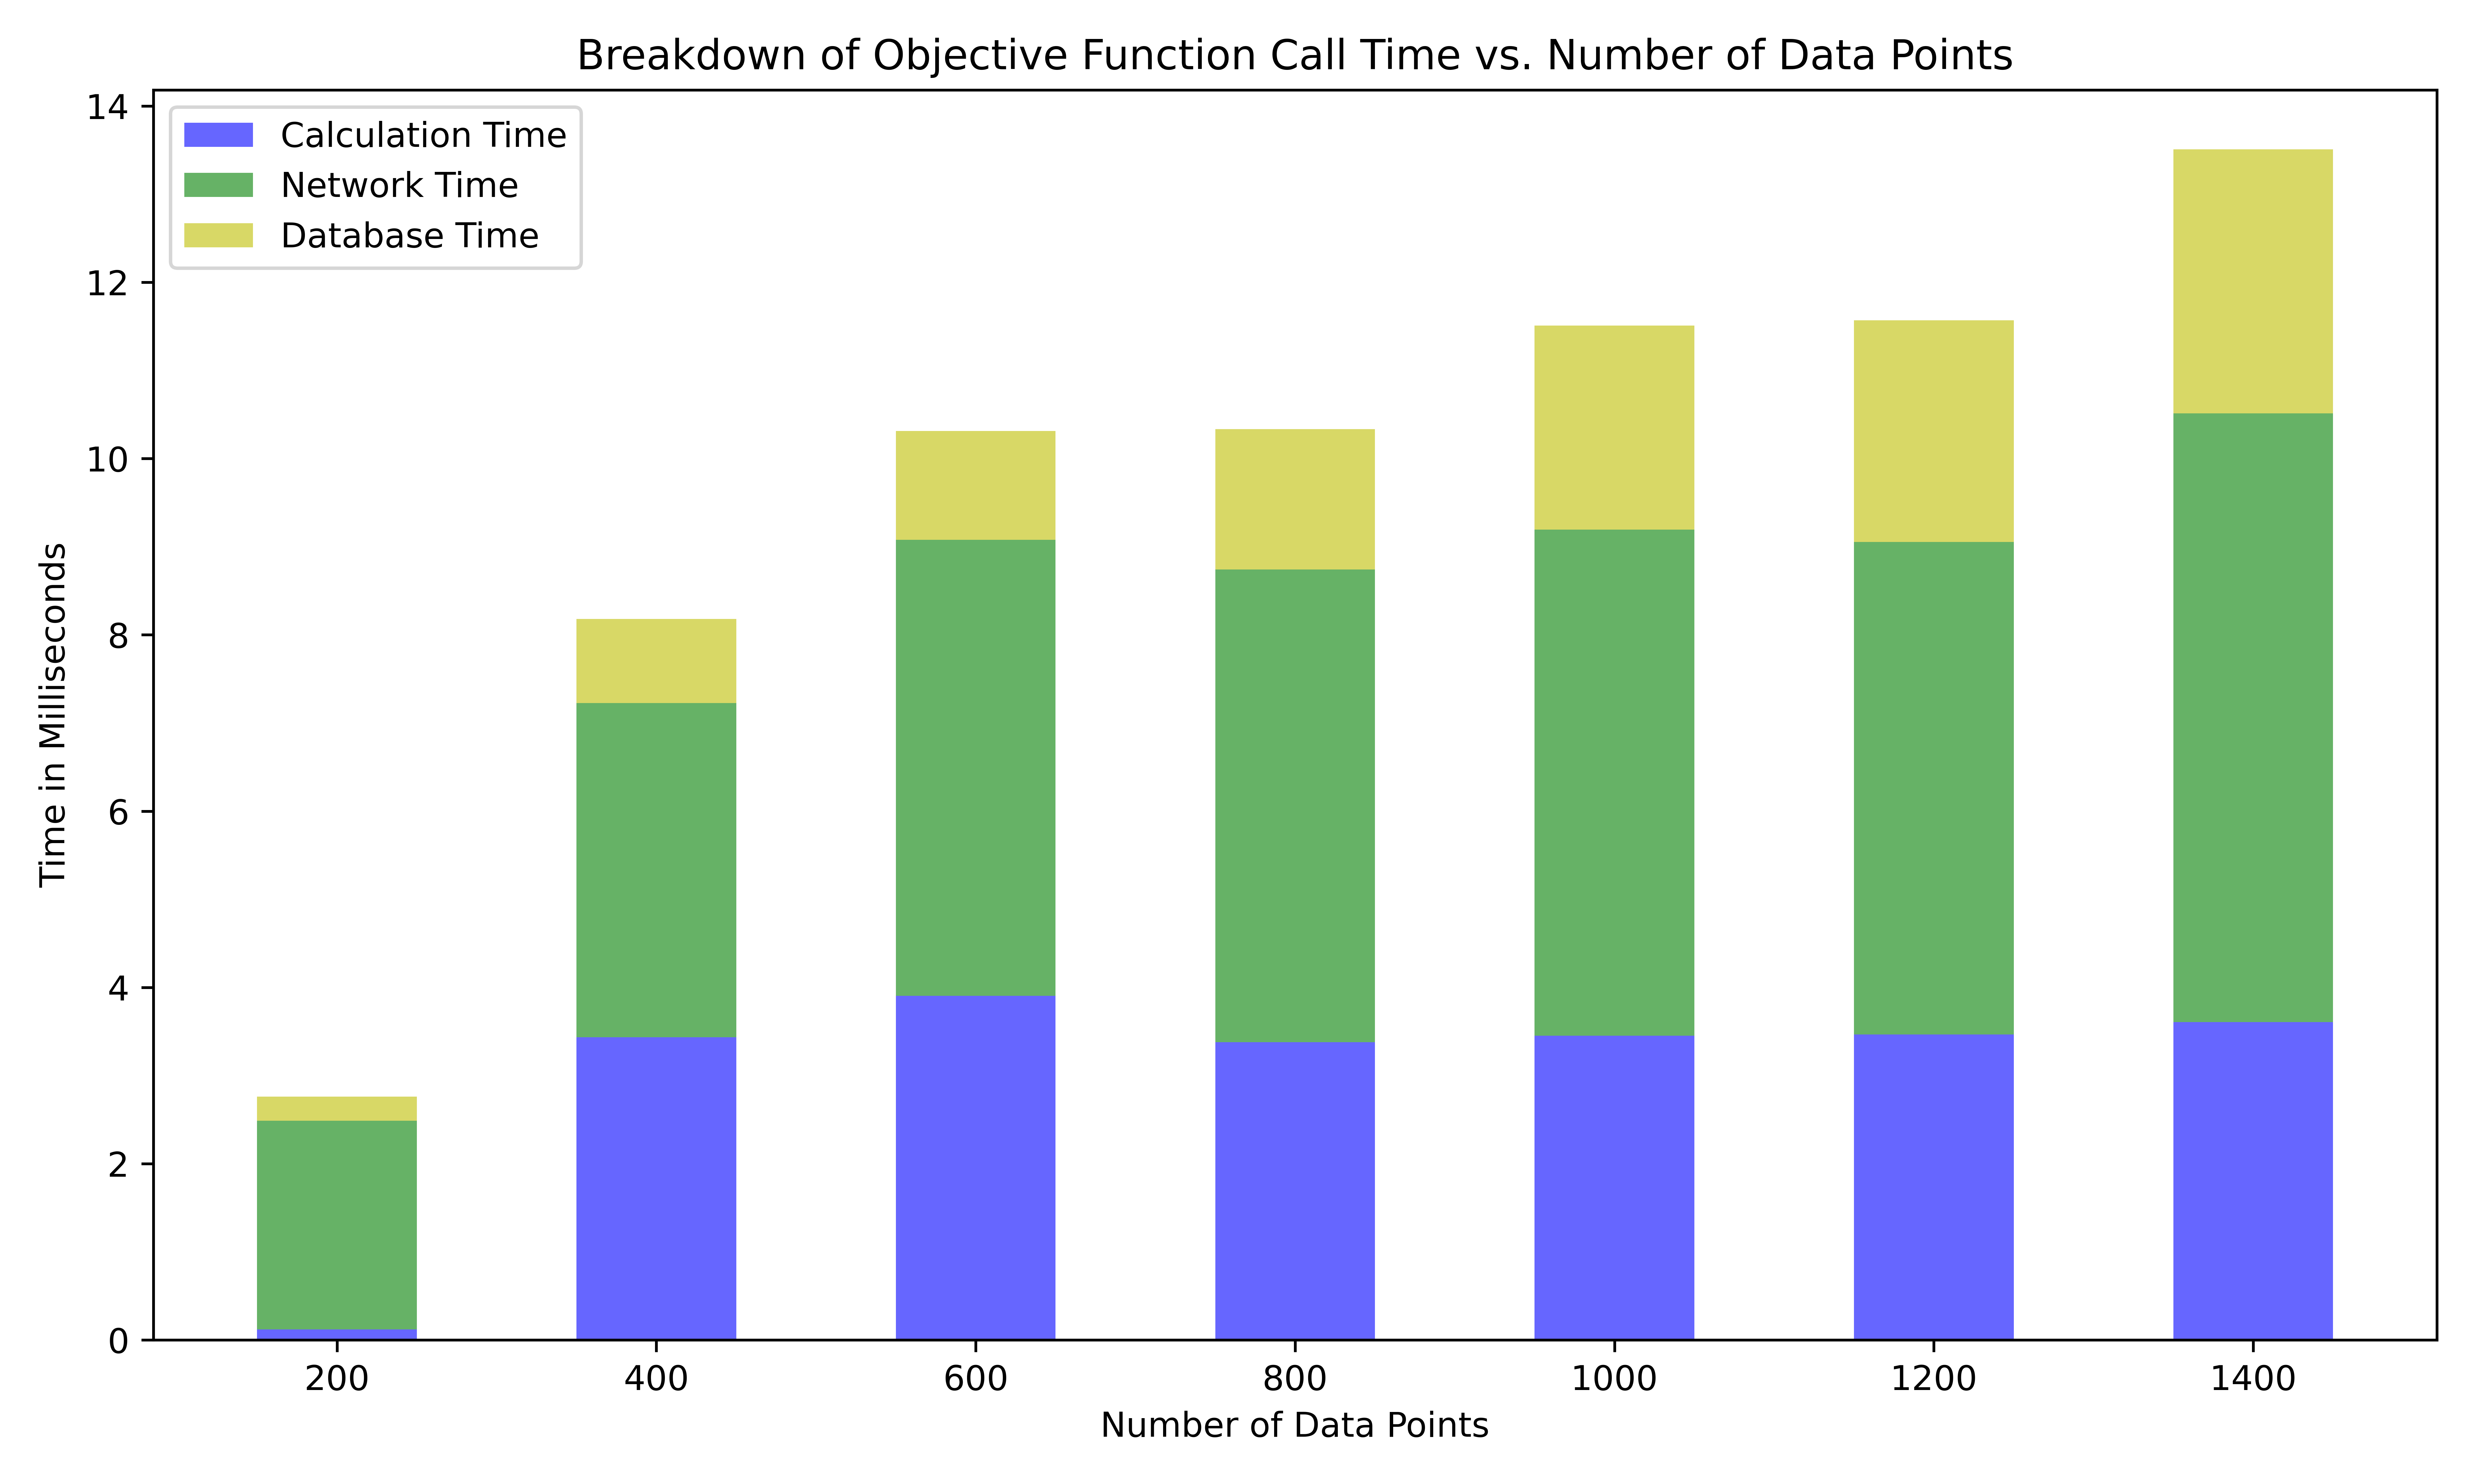
\includegraphics[width=\textwidth]{graphics/of_call_times_version1_cached.png}
%   \caption{Time it takes for a single call to the \emph{calc\_loss} endpoint of the \emph{ridge-loss} plugin for different dataset sizes for the first plugin-based implementation approach with caching.}
%   \label{fig:of_call_time_version1_cached}
% \end{figure}

% Figure \ref{fig:coparison_of_of_cached} shows a comparison between the total times it takes to get the loss across between the different implementations including a cached version of the first plugin-based implementation approach.

% \begin{figure}
%   \centering
%   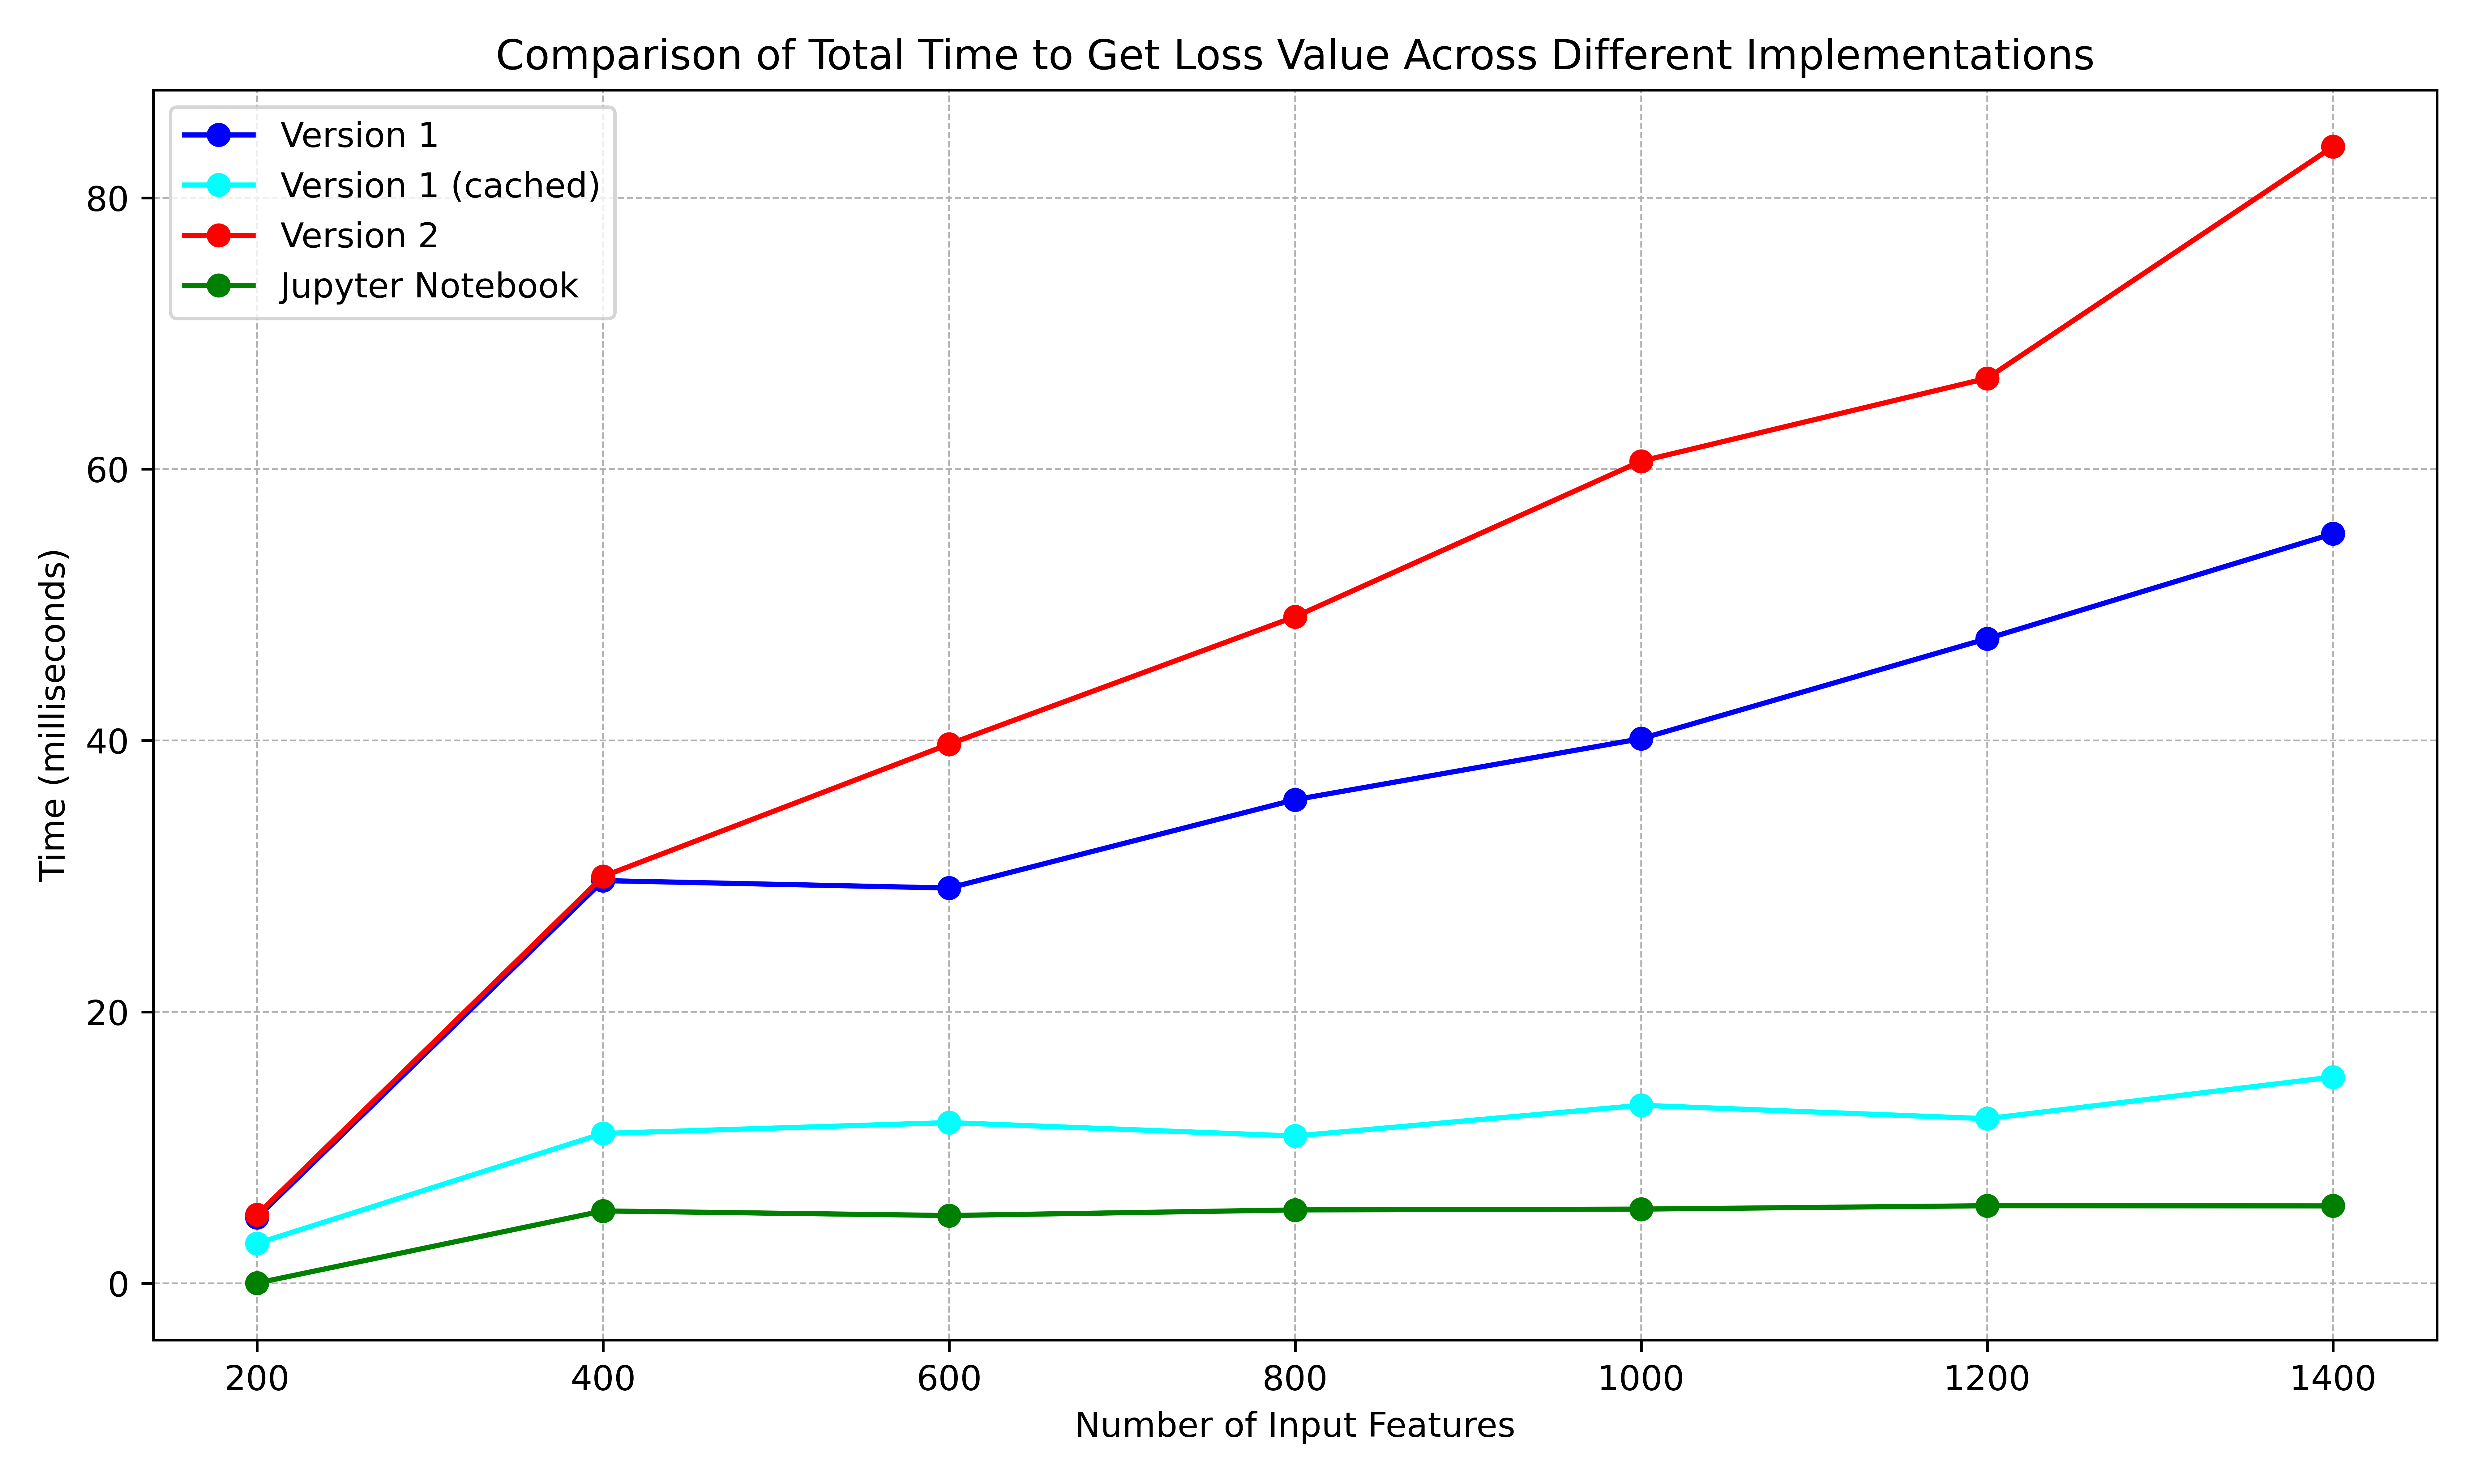
\includegraphics[width=\textwidth]{graphics/comparison_of_of_cached.png}
%   \caption{Comparison of the total time it takes to get the loss value across different implementations including a cached version of the first plugin-based implementation approach.}
%   \label{fig:coparison_of_of_cached}
% \end{figure}

% Finally, Figure \ref{fig:time_for_minimization} shows the total time it takes to complete the minimization process for the different implementations.
% The measurements for the plugin-based implementations do not include the time it takes a user to input data, but instead starts when the coordinator plugin calls the minimization endpoint of the minimizer plugin.

% \begin{figure}
%   \centering
%   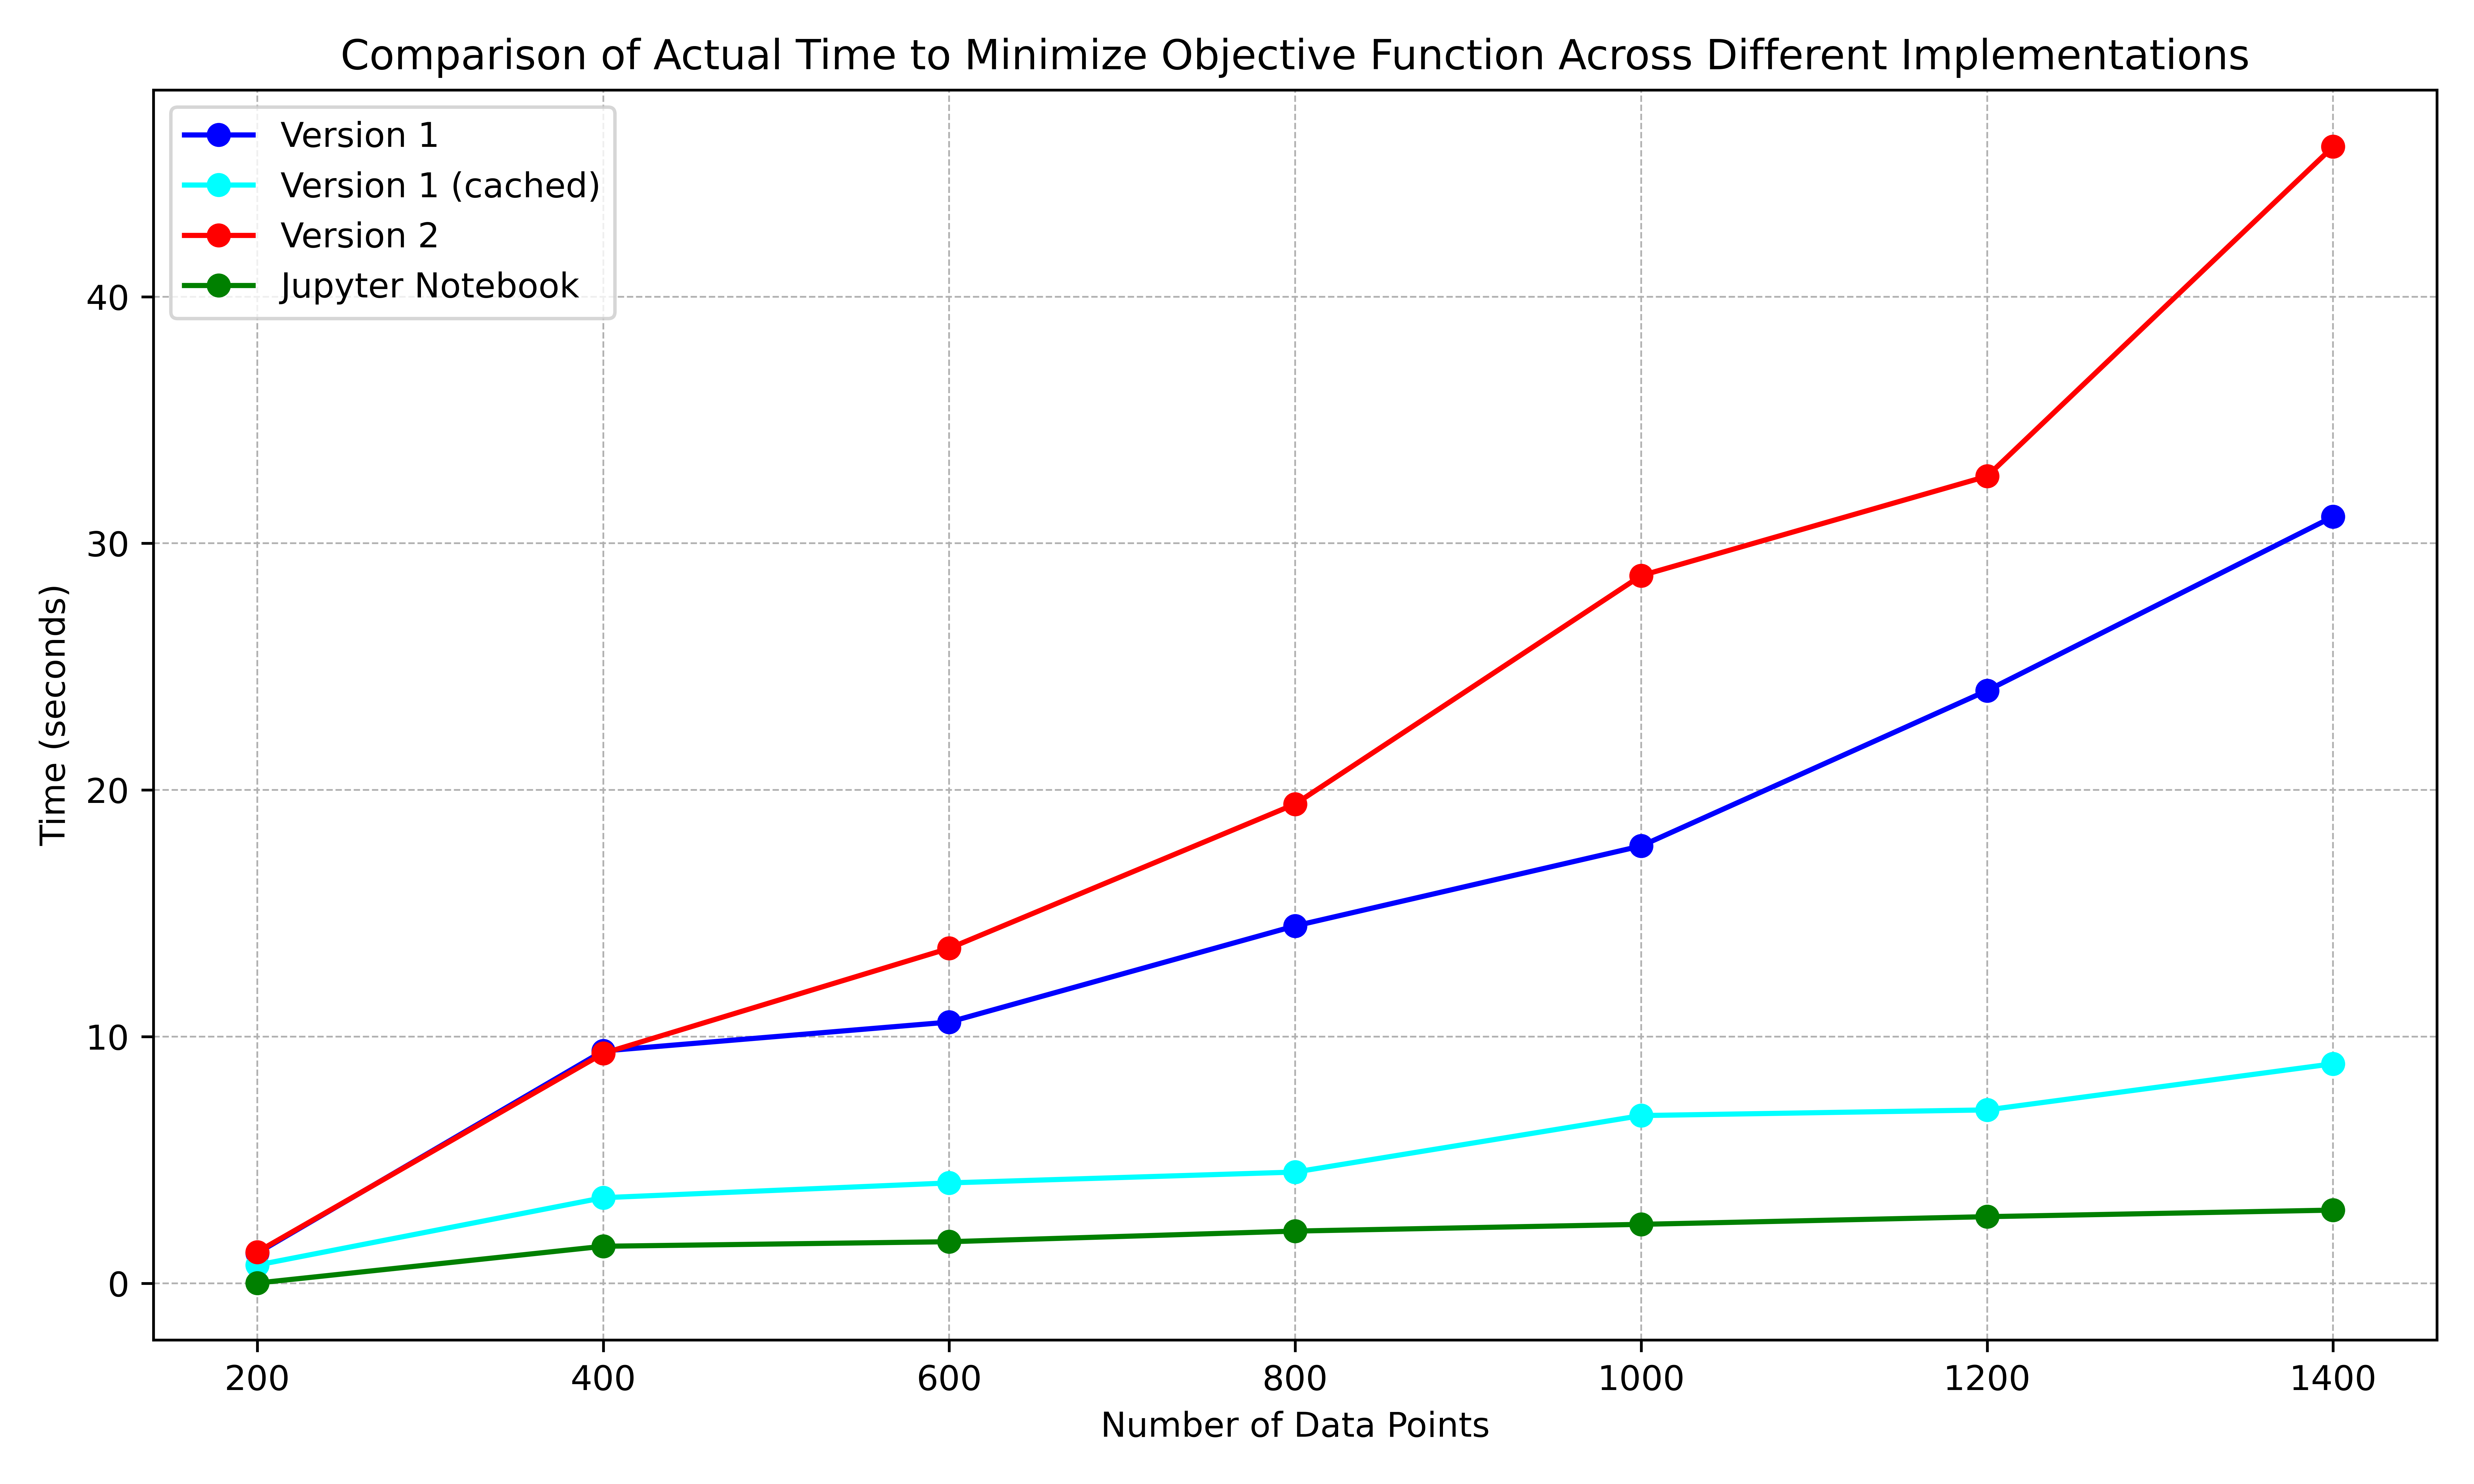
\includegraphics[width=\textwidth]{graphics/time_for_minimization.png}
%   \caption{Comparison of the total time it takes to complete the minimization process across different implementations.}
%   \label{fig:time_for_minimization}
% \end{figure}

\section{Interchangeability and Standardization of Plugins}
\label{sec:interchangeabilityOfPlugins}

This section explores if the plugins are interchangeable and if they adhere to the standards developed in this thesis.
The standards are defined in architecture Chapter \ref{chap:architecture} and the implementation Chapter \ref{chap:implementation}.
In summery the standards are:
\begin{description}
  \item[Metadata] Invocable plugins have to provide metadata that includes the interaction endpoints.
  \item[Interaction Endpoints] Invocable plugins have to provide interaction endpoints that adhere to the interaction endpoint schemas.
  \item[Callback Mechanisms] Invoking and invocable plugins have to provide the callback mechanism that is described in Section \ref{sec:implementationOfCallbacksToTheCoordinatorPlugin}.
  That includes the standard callback mechanism for the microfrontend invocation and the callback mechanism for the asynchronous minimization process.
  \item[Plugin Functionality] Each plugin has to implement the functionality it is supposed to implement as described in Section \ref{sec:decomposition}.
\end{description}

When a plugin fulfills all those standards it is interchangeable with other plugins that also fulfill the standards.
In the implementation part of the thesis all example plugins are implemented such that they fulfill the standards.
Therefore, they are interchangeable with each other, i.e. any minimizer plugin can be used with any \gls{of} plugin without the user having to change any code.
It is important to note thought that to leverage the gradient calculation that is provided by the \emph{neural-network} plugin, the \emph{scipy-minimizer-grad} plugin has to be used.

To make sure that there is no doubt that the plugins are interchangeable, we tested the combination of all minimizer plugins with all \gls{of} plugins and documented the results in Table \ref{table:interchangeability}.


\begin{table}[h!]
  \centering
  \begin{tabular}{|c|c|c|c|}
    \hline
    & \textbf{ridge-loss} & \textbf{hinge-loss} & \textbf{neural-network} \\
    \hline
    \textbf{scipy-minimizer} & \checkmark & \checkmark & \checkmark \\
    \hline
    \textbf{scipy-minimizer-grad} & \checkmark & \checkmark & \checkmark \\
    \hline
  \end{tabular}
  \caption{Compatibility between example implementation of plugins.}
  \label{table:interchangeability}
\end{table}



\section{Usability for Developers}
\label{sec:usabilityForDevelopers}

In this section the usability of the system for developers is explored.
The usability is shown by listing the steps a developer has to take to implement a new minimizer and \gls{of} plugin.
The first step is always to copy a already existing plugin into a new folder, since only a few lines of code have to be changed to provide new functionality.
At no point does a developer have to change any code of the coordinator plugin.

\subsection{Implementing a Minimizer Plugin}
\label{subsec:implementingAMinimizerPlugin}

In order to implement a new minimizer plugin, the developer has to follow these steps:

\begin{enumerate}
  \item Copy the \emph{scipy-minimizer} plugin into a new folder.
  \item Rename the plugin in the \emph{\_\_init\_\_.py} file.
  \item Add any needed hyperparameters to the \emph{MinimizerSetupTaskInputSchema} schema.
  \item Implement the minimization algorithm in the \emph{minimize\_task} function.
\end{enumerate}

\subsection{Implementing an Objective Function Plugin}
\label{subsec:implementingAnObjectiveFunctionPlugin}

In order to implement a new \gls{of} plugin, the developer has to follow these steps:

\begin{enumerate}
  \item Copy the \emph{ridge-loss} plugin into a new folder.
  \item Rename the plugin in the \emph{\_\_init\_\_.py} file.
  \item Add any needed hyperparameters to the \emph{HyperparamterInputSchema} schema.
  \item Implement the calculation for the number of input weights in the \emph{of\_pass\_data} endpoint.
  \item Implement the calculation of the loss function in the \emph{calc\_loss} endpoint.
\end{enumerate}


\chapter{Discussion}
\label{chap:discussion}

Interaciton endpoints
this concept has several advantages
* it allows for full interchangeability of plugins
* it allows the developer that want to interact with a plugin to know what endpoints are available and how to call them
* an alternatiev would be to return the url of available endpoitns after passing through the ui, now we can completely skip the ui alltogether and just call the endpoint directly

\section{Achievements and Contribution}
\label{sec:achievementsAndContribution}
\section{Limitations}
\label{sec:limitations}


\chapter{Conclusion and Outlook}
\label{chap:zusfas}

\section{Outlook}

\printbibliography

All links were last followed on October 15, 2023.

\appendix
\lstinputlisting[language=Python, caption={Source code for generating a sample test dataset for benchmarking with 1000 samples, 47 features, 10 noise and 1 target}., label=lst:generate_test_dataset]{code/ridge_loss_data.py}.

\pagestyle{empty}
\renewcommand*{\chapterpagestyle}{empty}
\Versicherung
\end{document}
